\documentclass[nobib,notoc,twoside,symmetric]{tufte-book}
\setcounter{tocdepth}{4}
\setcounter{secnumdepth}{4}

\usepackage{marginfix}
%to fix margins
\usepackage{multicol}
%for two-column.
\usepackage{CJKutf8}
%for mandarin

%\usepackage{scrextend} 
%\changefontsizes[11pt]{12pt}

\renewcommand{\footnotesize}{\small}

\geometry{a4paper,landscape,inner=30mm,top=15mm,bottom=10mm,headsep=\baselineskip,textwidth=170mm,marginparsep=8mm,marginparwidth=80mm,textheight=170mm,headheight=\baselineskip}

%\geometry{showframe}% for debugging purposes -- displays the margins

%\usepackage{stmaryrd}
%\usepackage{fontawesome}

\usepackage{amsmath,amsthm,amssymb,amsfonts}
\theoremstyle{definition}
\newtheorem{theorem}{Theorem}[section]
\newtheorem*{theorem*}{Theorem}
\newtheorem{corollary}[theorem]{Corollary}
\newtheorem{lemma}[theorem]{Lemma} 
\newtheorem{proposition}[theorem]{Proposition}
\newtheorem{conj}[theorem]{Conjecture}
\newtheorem{defn}[theorem]{Definition}
\newtheorem{fact}[theorem]{Fact} 
\newtheorem{example}[theorem]{Example} 
\newtheorem{examples}[theorem]{Examples}
\newtheorem{example*}[theorem]{Example*}
\newtheorem{examples*}[theorem]{Examples*}
\newtheorem{remark}[theorem]{Remark}
\newtheorem{remark*}[theorem]{Remark*}
\newtheorem{question}[theorem]{Question}
\newtheorem{assumption}[theorem]{Assumption}
\newtheorem{conjecture}[theorem]{Conjecture}
\newtheorem{convention}[theorem]{Convention}
\newtheorem{justification}[theorem]{Justification} 
\newtheorem{construction}[theorem]{Construction}
\newtheorem{rem}[theorem]{Reminder}
\newtheorem{intuition}[theorem]{Intuition}
\newtheorem{term}[theorem]{Terminology}
\newtheorem{scholium}[theorem]{Scholium}
\newtheorem{requirement}[theorem]{Requirement}
\newtheorem{notation}[theorem]{Notation}
\newtheorem{refinement}[theorem]{Refinement}
\newtheorem{thesis}[theorem]{Thesis}

%for fonts
\usepackage{newpxtext}
%\usepackage[fracspacing]{newpxmath}
\linespread{1.05}

\usepackage{tikz-cd}
\usepackage{macros/tikzfig}
\usepackage{macros/quiver}
\input{macros/thesis.tikzstyles}

% Set up the images/graphics package
\usepackage{graphicx}
\setkeys{Gin}{width=\linewidth,totalheight=\textheight,keepaspectratio}
\graphicspath{{graphics/}}

\title{String diagrams for text}
\author[V.W.]{Vincent Wang-Ma\'{s}cianica}
\date{\today}

% The following package makes prettier tables.  We're all about the bling!
\usepackage{booktabs}

% The units package provides nice, non-stacked fractions and better spacing
% for units.
\usepackage{units}

% The fancyvrb package lets us customize the formatting of verbatim
% environments.  We use a slightly smaller font.
\usepackage{fancyvrb}
\fvset{fontsize=\normalsize}

% Small sections of multiple columns
\usepackage{multicol}

% Squares
\usepackage{stix}

% Provides paragraphs of dummy text
\usepackage{lipsum}

% These commands are used to pretty-print LaTeX commands
\newcommand{\doccmd}[1]{\texttt{\textbackslash#1}}% command name -- adds backslash automatically
\newcommand{\docopt}[1]{\ensuremath{\langle}\textrm{\textit{#1}}\ensuremath{\rangle}}% optional command argument
\newcommand{\docarg}[1]{\textrm{\textit{#1}}}% (required) command argument
\newenvironment{docspec}{\begin{quote}\noindent}{\end{quote}}% command specification environment
\newcommand{\docenv}[1]{\textsf{#1}}% environment name
\newcommand{\docpkg}[1]{\texttt{#1}}% package name
\newcommand{\doccls}[1]{\texttt{#1}}% document class name
\newcommand{\docclsopt}[1]{\texttt{#1}}% document class option name

\usepackage{bussproofs}

\usepackage{xcolor}
\usepackage{xspace}
\def\bB{\begin{color}{blue}}
\def\bO{\begin{color}{orange}}
\def\bG{\begin{color}{green}}
\def\bM{\begin{color}{magenta}}
\def\e{\end{color}\xspace}

%For chesspieces
\usepackage{skak}

%For Brakets
\usepackage{physics}

\usepackage{xspace} 
%\usepackage{enumerate}
\usepackage{color} 
\def\bR{\begin{color}{red}}
\def\bB{\begin{color}{blue}}
\def\e{\end{color}\xspace}

%\usepackage{tocloft}
%\cftsetindents{section}{0em}{2em}
%\cftsetindents{subsection}{0em}{2em}
%\renewcommand\cfttoctitlefont{\hfill\Large\bfseries}
%\renewcommand\cftaftertoctitle{\hfill\mbox{}}

\begin{document}

\maketitle% this prints the handout title, author, and date

%\begin{fullwidth}
%\begin{multicols}{2}
\tableofcontents\marginnote{(Acknowledgements will go in a margin note here.)}

\chapter{Text circuits for syntax}\label{chapter:textcircuits}
We want to establish that there is a systematic correspondence between text circuits and grammatically acceptable text, which would allow us to use text circuits as a generative grammar without further justification. First we show that context-free grammars, string-rewrite systems, and tree-adjoining grammars are all special cases of higher-dimensional rewriting systems called weak $n$-categories. Then we provide a "circuit-growing" grammar in terms of a weak $n$-categorical signature that simultaneously generates strings of grammatically acceptable text and its "deep structure" in terms of text circuits, from which we obtain the desired correspondence between text circuits and text. We close with demonstrations of how the syntactic theory of text circuits may be modified and expanded, and a brief note on how text circuits relate to Montague's "Universal Grammar".
\newpage
\section{An introduction to weak n-categories for formal linguists}

Geometrically, a set is a collection of labelled zero-dimensional points. A category is a collection of one-dimensional labelled arrows upon a set of zero-dimensional points (that satisfy certain additional conditions, such as having identity morphisms and associativity of composition.) Naturally, we might ask what happens when we generalise to more dimensions, asking for two-dimensional somethings going between one-dimensional arrows, and three-dimensional somethings going between two-dimensional somethings, and so on. This is the gist of an $n$-category, where $n$ is a positive integer denoting dimension.\\

There is a fork in the road in generalisation. First, different choices of what n-dimensional somethings could be give different conceptions of $n$-category, because there are multiple mathematically well-founded choices for filling in the blank of \texttt{points, lines, ???}. Simplices, cubical sets, and globular sets are three common options; though the names are fancy, they correspond to triangular, cubical, and circular families of objects indexed by dimension.

\[placeholder\]

Second, there is a distinction between \emph{strict} and \emph{weak} $n$-categories. Just as in regular or $1$-category theory we are interested in objects up to isomorphism rather than equality -- because isomorphic objects in a category are as good as one another -- lifting this philosophy to $n$-categories gives us \emph{weak} $n$-categories. In a strict $k$-category, all of the $j$-dimensional morphisms for $j > k$ are identity-equalities. In a weak $k$-category, all equalities for dimensions $j > k$ are replaced by isomorphisms all the way up: which means that a $k$-equality $\alpha = \beta$ in the strict setting is replaced by a pair of $k+1$-morphisms witnessing the isomorphism of $\alpha$ and $\beta$, and that pair of $k+1$-morphisms has a pair of $k+2$ morphisms witnessing that they are $k+1$-isomorphic, and so on for $k+3$ and all the way up. Unsurprisingly, strict $n$-categories are easy to formalise, and weaks $n$-categories are hard. A conjecture or guiding principle like the Church-Turing thesis holds for weak $n$-categories that they should all be equivalent to one another, whatever equivalence means.\\

Mathematicians, computer scientists, and physicists may have good reasons to work with weak $n$-categories [], but what is the value proposition for formal linguists? A philosophical draw for the formal semanticist is that insofar as semantics is synonymy -- the study of when expressions are equivalent -- weak $n$-categories are an exquisite setting to control and study sameness in terms of meta-equivalences. A practical draw for the formal syntactician is that weak $n$-categories provide a natural setting to model generic rewriting systems, and that is what we will focus on here. In this setting we will introduce weak $n$-categories in the \texttt{homotopy.io} formulation, along the way showing how they provide a common setting to formalise string-rewrite and tree-adjoining grammars, setting the stage for us to specify a circuit-adjoining grammar for text circuits later on. 

\subsection{String-rewrite systems as 1-object-2-categories}

Say we have an alphabet $\Sigma := \{\textcolor{green}{\alpha}, \textcolor{orange}{\beta}, \textcolor{cyan}{\gamma}\}$. Then the Kleene-star $\Sigma^*$ consists of all strings (including the empty string $\varepsilon$) made up of $\Sigma$, and we consider formal languages on $\Sigma$ to be subsets of $\Sigma^*$. Another way of viewing $\Sigma^*$ is as the free monoid generated by $\Sigma$ under the binary concatenation operation $(\_ \ \cdot \ \_)$ which is associative and unital with unit $\varepsilon$, the empty string. Associativity and unitality are precisely the conditions of composition of morphisms in categories, so we have yet another way to express $\Sigma^*$ as a finitely presented category; we consider a category with a single object $\star$, taking $\varepsilon$ to be the identity morphism $\textbf{1}_\star$ on the single object, and we ask for the category obtained when we consider the closure under composition of three non-identity morphisms $\textcolor{green}{\alpha}, \textcolor{orange}{\beta}, \textcolor{cyan}{\gamma}: \star \rightarrow \star$. In this category, every morphism $\star \rightarrow \star$ corresponds to a string in $\Sigma^*$. We illustrate this example in the margins. A string-rewrite system additionally consists of a finite number of string-transformation rules. Building on our example, we might have a named rule $\textcolor{magenta}{R}: \textcolor{green}{\alpha} \mapsto \textcolor{orange}{\beta} \cdot \textcolor{cyan}{\gamma}$, which we illustrate in Figure \ref{fig:ruleR}.\\

\begin{marginfigure}
\centering
\[\tikzfig{ncat/flower1}\]
\caption{The category in question can be visualised as a commutative diagram.}
\end{marginfigure}

\begin{marginfigure}
\centering
\[\resizebox{\textwidth}{!}{\tikzfig{ncat/table1}}\]
\caption{When there are too many generating morphisms, we can instead present the same data as a table of $n$-cells; there is a single 0-cell $\star$, and three non-identity 1-cells corresponding to $\textcolor{green}{\alpha}, \textcolor{orange}{\beta}, \textcolor{cyan}{\gamma}$, each with source and target 0-cells $\star$. Typically identity morphisms can be omitted from tables as they come for free. Observe that composition of identities enforces the behaviour of the empty string, so that for any string $x$, we have $\epsilon \cdot x = x = \epsilon \cdot x$.}
\end{marginfigure}

\begin{marginfigure}
\centering
\[\tikzfig{ncat/cstring1}\]
\caption{For a concrete example, we can depict the string $\textcolor{green}{\alpha} \cdot \textcolor{cyan}{\gamma} \cdot \textcolor{cyan}{\gamma} \cdot \textcolor{orange}{\beta}$ as a morphism in a commuting diagram.}
\end{marginfigure}

\begin{marginfigure}
\centering
\[\tikzfig{ncat/string1}\]
\caption{The string-diagrammatic view, where $\star$ is treated as a wire and morphisms are treated as boxes or dots is an expression of the same data under the Poincar\'{e} dual.}
\end{marginfigure}

\begin{marginfigure}\label{fig:ruleR}
\centering
\[\tikzfig{ncat/poindual}\]
\caption{We can visualise the rule as a commutative diagram where $\textcolor{magenta}{R}$ is a 2-cell between the source and target 1-cells. Just as 1-cells are arrows between 0-cell points in a commuting diagram, a 2-cell can also be conceptualised as a directed surface from a 1-cell to another. Taking the Poincar\'{e} dual of this view gives us a string diagram for the 2-cell $\textcolor{magenta}{R}$.}
\end{marginfigure}

\newthought{We consider rewrites to be equivalent, but not equal.} In a string-rewrite system, rewrites are applied one at a time. This means that even for our simple example, there are two possible rewrites from $\textcolor{green}{\alpha} \cdot \textcolor{green}{\alpha}$ to obtain $\textcolor{orange}{\beta} \cdot \textcolor{cyan}{\gamma} \cdot \textcolor{orange}{\beta} \cdot \textcolor{cyan}{\gamma}$. Here are the two rewrites viewed in two equivalent ways, first on the left informally where strings are nodes in a graph and rewrites are labelled transitions and secondly on the right as two distinct commuting 2-diagrams.

\[\resizebox{0.8\textwidth}{!}{\tikzfig{ncat/2ways}}\]

What should we say about how these two different rewrites relate to each other? Let's say Alice is a formal linguist who is only interested in what strings are reachable from others by rewrites -- this is \emph{de rigeur} when we consider formal languages to be subsets of $\Sigma^*$. She might be happy to declare that these two rewrites are simply equal; categorically this is tantamount to her declaring that any two 2-cells in the 1-object-2-category that share the same source and target are in fact the same, or equivalently, that any $n$-cells for $n \geq 3$ are identities. In fact, what Alice really cares to have is a category where the objects are strings from $\Sigma^*$, and the morphisms are a reachability relation by rewrites; this category is \emph{thin}, in that there is at most one arrow between each pair of objects, which forgets what rewrites are applied.

\[\tikzfig{ncat/thinalice}\]

Let's say Bob is a different sort of formal linguist who wants to model the two rewrites as nonequal but equivalent, with some way to keep track of how different equivalent rewrites relate to one another. Bob might want this for example because he wants to show that head-first rewrite strategies are the same as tail-first, so he wants to keep the observation that the two rewrites are equivalent in that they have the same source and target, while keeping the precise order of rewrites distinct. This order-independence of disjoint or non-interfering rewrites is reflected in the interchange law for monoidal categories, which in the case of our example is depicted as:

\[\tikzfig{ncat/bobfat}\]

In fact, Bob gets to express a new kind of rewrite in the middle: the kind where two non-conflicting rewrites happen \emph{concurrently}. The important aspect of Bob's view over Alice's is that equalities have been replaced by isomorphisms between syntactically inequal rewrites. This demotion of equalities to isomorphisms means that Bob is dealing with a \emph{weak} 1-object-2-category; Bob does have 3-cells that relate different 2-cells with the same source and target, but all of Bob's $n$-cells for $n \geq 3$ are isomorphisms, rather than equalities.

\subsection{A context free grammar to generate \texttt{Alice sees Bob quickly run to school}}

We can describe a context-free grammar with the same combinatorial rewriting data that specifies planar string diagrams as we have been illustrating so far. One aspect of rewrite systems we adapt for now is the distinction between terminal and nonterminal symbols; terminal symbols are those after which no further rewrites are possible. We capture this string-diagrammatically by modelling terminal rewrites as 2-cells with target equal to the 1-cell identity of the 0-cell $\star$, which amounts to graphically terminating a wire. The generators subscripted $L$ (for \emph{label} or \emph{leaf}) correspond to terminals of the CFG, and represent a family of generators indexed by a lexicon for the language. The generators subscripted $i$ (for \emph{introducing a type}) correspond to rewrites of the CFG.

\[\scalebox{0.5}{\tikzfig{tree2gate/cfg/cfgsignature}}\]

Consider the sentence \texttt{Alice sees Bob quickly run to school}, which we take to be generated by the following context-free grammar derivation, read from left-to-right. We additionally depict the breakdown of the derivation in terms of rewrites of lower dimension from our signature.

\[\scalebox{0.5}{\tikzfig{tree2gate/cfg/bigcfgbreakdown}}\]

\[\scalebox{0.3}{\tikzfig{tree2gate/workedexample/bigcfg}}\]

\subsection{Tree Adjoining Grammars}

Here is a formal but unenlightening definition of \emph{elementary} tree adjoining grammars which we will convert to diagrams. We will deal with the extensions of links and local constraints to adjoining shortly.

\begin{defn}[\emph{Elementary} Tree Adjoining Grammar: Classic Computer Science style]
*A \textbf{TAG} is a tuple $(\mathcal{N}, \mathcal{N}^\downarrow, \mathcal{N}^*, \Sigma, \mathcal{I}, \mathcal{A})$. These denote, respectively:
\begin{itemize}
	\item{ The \emph{non-terminals}:
		\begin{itemize}
			\item{A set of \emph{non-terminal symbols} $\mathcal{N}$ -- these stand in for grammatical types such as $\texttt{NP}$ and $\texttt{VP}$.}
			\item{A bijection $\downarrow: \mathcal{N} \rightarrow \mathcal{N}^\downarrow$ which acts as $\texttt{X} \mapsto \texttt{X}^\downarrow$. Nonterminals in $\mathcal{N}$ are sent to marked counterparts in $\mathcal{N}^\downarrow$, and the inverse sends marked nonterminals to their unmarked counterparts. These markings are \emph{substitution markers}, which are used to indicate when certain leaf nodes are valid targets for a substitution operation -- discussed later.}
			\item{A bijection $*: \mathcal{N} \rightarrow \mathcal{N}^*$ -- the same idea as above. This time to mark \emph{foot nodes} on auxiliary trees, which is structural information used by the adjoining operation -- discussed later.}
	\end{itemize}
	}
	\item{A set of \emph{terminal symbols} $\Sigma$ -- these stand in for the words of the natural language being modelled.}
	\item{The \emph{elementary trees}:
		\begin{itemize}
			\item{A set of \emph{initial trees} $\mathcal{I}$, which satisfy the following constraints:
			\begin{itemize}
				\item{The interior nodes of an initial tree must be labelled with nonterminals from $\mathcal{N}$}
				\item{The leaf nodes of an initial tree must be labelled from $\Sigma \cup \mathcal{N}^{\downarrow}$}
			\end{itemize}
			}
	\item{A set of \emph{auxiliary trees} $\mathcal{A}$, which satisfy the following constraints:
		\begin{itemize}
			\item{The interior nodes of an auxiliary tree must be labelled with nonterminals from $\mathcal{N}$}
			\item{Exactly one leaf node of an auxiliary tree must be labelled with a foot node $\texttt{X}^{*} \in \mathcal{N}^{*}$; moreover, this labelled foot node must be the marked counterpart of the root node label of the tree.}
			\item{All other leaf nodes of an auxiliary tree are labelled from $\Sigma \cup \mathcal{N}^{\downarrow}$}
		\end{itemize}
		}
	\end{itemize}
	}
\end{itemize}
There are two operations to build what are called \emph{derived trees} from elementary and derived trees. These operations are called \emph{substitution} and \emph{adjoining}.
\begin{itemize}
	\item{\emph{Substitution} replaces a substitution marked leaf node $\texttt{X}^\downarrow$ in a tree $\alpha$ with another tree $\alpha'$ that has $\texttt{X}$ as a root node.}
	\item{\emph{Adjoining} takes auxiliary tree $\beta$ with root and foot nodes $\texttt{X},\texttt{X}^\star$, and a derived tree $\gamma$ at an interior node $\texttt{X}$ of $\gamma$. Removing the $\texttt{X}$ node from $\gamma$ separates it into a parent tree with an $\texttt{X}$-shaped hole for one of its leaves, and possibly multiple child trees with \texttt{X}-shaped holes for roots. The result of adjoining is obtained by identifying the root of $\beta$ with the $\texttt{X}$-context of the parent, and making all the child trees children of $\beta$s foot node $\texttt{X}^\star$.}
\end{itemize}
\end{defn}

The essence of a tree-\emph{adjoining} grammar is as follows: whereas for a CFG one grows the tree by appending branches and leaves at the top of the tree (substitution), in a TAG one can also sprout subtrees from the middle of a branch (adjoining). Now we show that this gloss is more formal than it sounds, by the following steps. First we show that the 2-categorical data of a CFG can be transformed into 3-categorical data -- which we call \emph{Leaf-Ansatz} -- which presents a rewrite system that obtains the same sentences as the CFG, by a bijective correspondence between composition of 2-cells in the CFG and constructed 3-cells in the leaf-ansatz. These 3-cells in the leaf ansatz correspond precisely to the permitted \emph{substitutions} in a TAG. Then we show how to model \emph{adjoining} as 3-cells. Throughout we work with a running example, the CFG grammar introduced earlier.

\begin{construction}[Leaf-Ansatz of a CFG]
Given a signature $\mathfrak{G}$ for a CFG, we construct a new signature $\mathfrak{G}'$ which has the same 0- and 1-cells as $\mathfrak{G}$. See the dashed magenta arrows in the schematic below. For each 1-cell wire type $\texttt{X}$ of $\mathfrak{G}$, we introduce a \emph{leaf-ansatz} 2-cell $\texttt{X}^\downarrow$. For each leaf 2-cell $\texttt{X}_L$ in $\mathfrak{G}$, we introduce a renamed copy $\texttt{X}'_L$ in $\mathfrak{G}'$. Now see the solid magenta arrows in the schematic below. We construct a 3-cell in $\mathfrak{G}'$ for each 2-cell in $\mathfrak{G}$, which has the effect of systematically replacing open output wires in $\mathfrak{G}$ with leaf-ansatzes in $\mathfrak{G}'$.
\[\scalebox{0.5}{\tikzfig{tree2gate/tag/CFGtoTAGpattern}}\]
\end{construction}

\begin{example}
The leaf-ansatz construction just makes formal the following observation: there are multiple equivalent ways of modelling terminal symbols in a rewrite system considered string-diagrammatically. One way (which we have already done) is to treat non-terminals as wires and terminals as effects, so that the presence of an open wire available for composition visually indicates non-terminality. Another (which is the leaf-ansatz construction) treats all symbols in a rewrite system as leaves, where bookkeeping the distinction between (non-)terminals occurs in the signature. So for a sentence like \texttt{Bob drinks}, we have the following derivations that match step for step in the two ways we have considered.
\[\scalebox{0.5}{\tikzfig{tree2gate/tag/leafansatzintuition}}\]
\end{example}

\begin{proposition}[Leaf-ansatzes of CFGs are precisely TAGs with only initial trees and substitution]\label{prop:cfgastag1}
\begin{proof}
By construction. Consider a CFG given by 2-categorical signature $\mathfrak{G}$, with leaf-ansatz signature $\mathfrak{G}'$. The types $\texttt{X}$ of $\mathfrak{G}$ become substitution marked symbols $\texttt{X}^{\downarrow}$ in $\mathfrak{G}'$. The trees $\texttt{X}_i$ in $\mathfrak{G}$ become initial trees $\texttt{X}^0$ in $\mathfrak{G}'$. The 3-cells $\texttt{X}_s$ of $\mathfrak{G}'$ are precisely substitution operations corresponding to appending the 2-cells $\texttt{X}_i$ of $\mathfrak{G}$.
\end{proof}
\end{proposition}

\begin{example}[Leaf-ansatz signature of \texttt{Alice sees Bob quickly run to school} CFG]
\[\scalebox{0.5}{\tikzfig{tree2gate/tag/CFGasTAGsign}}\]
\end{example}

\begin{example}[Adjoining is sprouting subtrees in the middle of branches]
One way we might obtain the sentence \texttt{Bob runs to school} is to start from the simpler sentence \texttt{Bob runs}, and then refine the verb \texttt{runs} into \texttt{runs to school}. This refinement on part of an already completed sentence is not permitted in CFGs, since terminals can no longer be modified. The adjoining operation of TAGs gets around this constraint by permitting rewrites in the middle of trees, as follows:
\[\scalebox{0.5}{\tikzfig{tree2gate/tag/3compareintuition}}\]
\end{example}

\begin{example}[TAG signature of \texttt{Alice sees Bob quickly run to school}]
The highlighted 2-cells are auxiliary trees that replace CFG 2-cells for verbs with sentential complement, adverbs, and adpositions. The highlighted 3-cells are the tree adjoining operations of the auxiliary trees.
\[\scalebox{0.5}{\tikzfig{tree2gate/tag/tagsignature}}\]
\end{example}

The construction yields as a corollary an alternate proof of Theorem [Joshi 6.1.1...]...

\begin{corollary}
For every context-free grammar $\mathfrak{G}$ there exists a tree-adjoining grammar $\mathfrak{G}'$ such that $\mathfrak{G}$ and $\mathfrak{G}'$ are strongly equivalent -- both formalisms generate the same set of strings (weak equivalence) and the same abstract syntactic structures (in this case, trees) behind the strings (strong equivalence).
\begin{proof}
Proposition \ref{prop:cfgastag1} provides one direction of both equivalences. For the other direction, we have to show that each auxiliary tree (a 2-cell) and its adjoining operation (a 3-cell) in $\mathfrak{G}'$ corresponds to a single 2-cell tree of some CFG signature $\mathfrak{G}$, which we demonstrate by construction. See the example above; the highlighted 3-cells of $\mathfrak{G}'$ are obtained systematically from the auxiliary 2-cells as follows: the root and foot nodes $\texttt{X},\texttt{X}^\star$ indicate which wire-type to take as the identity in the left of the 3-cell, and the right of the 3-cell is obtained by replacing all non-$\texttt{X}$ open wires $\texttt{Y}$ with their leaf-ansatzes $\texttt{Y}^\downarrow$. This establishes a correspondence between any 2-cells of $\mathfrak{G}$ considered as auxiliary trees in $\mathfrak{G}'$.
\end{proof}
\end{corollary}

\subsection{Tree adjoining grammars with local constraints}

The usual conception of TAGs includes two extensions to the basic definition presented above. First, there may be \emph{local constraints} on adjoining, which only allows certain trees to be adjoined at certain nodes. Second, TAGs may have links, which are extra edges between nodes obeying a c-command condition. Here we deal with local constraints; dealing with links requires the introduction of braiding.

\begin{defn}[TAG with local constraints: CS-style] [Joshi]
$G = (I,A)$ is a TAG with local constraints if for each node $n$ and each tree $t$, exactly one of the following constraints is specified:
\begin{enumerate}
\item{Selective adjoining (SA): Only a specified subset $\bar{\beta} \subseteq A$ of all auxiliary trees are adjoinable at $n$.}
\item{Null adjoining (NA): No auxiliary tree is adjoinable at the node $n$.}
\item{Obligatory Adjoining (OA): At least one out of all the auxiliary trees adjoinable at $n$ must be adjoined at $n$.}
\end{enumerate}
\end{defn}

The $n$-categorical approach easily accommodates local constraints. For (SA), whereas before we take the source of adjoining rewrites to be identities, we can instead introduce ansatz endomorphisms that are rewritable to the desired subsets. For (NA), we assert that identities have no rewrites (NA). For (OA), we can make a distinction between finished and unfinished derivations, where we require that unfinished derivations are precisely those that still contain an obligatory-rewrite endomorphism.

\begin{example}[Selective and null adjoining diagrammatically]
The below is a reproduction of Example 2.5 of [Joshi] which demonstrates the usage of selective and null adjoining. The notation from [Joshi] is presented first, followed by their corresponding representations in an $n$-categorical signature. The initial tree is presented as a 2-cell where the (SA) rules are rewritable nodes, that serve as sources of rewrites in the 3-cell presentations of the auxiliary trees.
\[\resizebox{\textwidth}{!}{\tikzfig{tree2gate/tag/ex25}}\]
\end{example}

\begin{example}[Obligatory adjoining diagrammatically]
The below is a reproduction of Example 2.11 of [Joshi] which demonstrates the usage of obligatory adjoining, marked orange. The notation from [Joshi] is presented first, followed by their corresponding representations in an $n$-categorical signature. The initial tree is presented as a 2-cell where the (OA) rule is given its own 2-cell, which is the source of rewrites in 3-cell presentations of auxiliary trees. We may capture the obligatory nature of the rewrite by asking that finished derivations contain no instance of the orange 2-cell.
\[\resizebox{\textwidth}{!}{\tikzfig{tree2gate/tag/ex211}}\]
\end{example}

\subsection{Braiding, symmetries, and suspension}

Before we can model TAGs with links, we must introduce the concepts of braiding and symmetries, which we have seen in the diagrammatic setting already as wires twisting past one another. In our current setting of 1-object-3-categories for TAGs, the diagrams we are dealing with are all planar -- i.e. wires may not cross -- but this is a restriction we must overcome when we are dealing with links.\\

First we observe that in a 1-object-2-categorical setting, a morphism from the identity $\varepsilon$ on the base object $\star$ to itself would, in our analogy with string-rewrite systems, be a rewrite from the empty string to itself. For example, a rewrite $R$ may introduce a symbol from the empty string and then delete it. A rewrite $S$ may create a pair of symbols from nothing and then annihilate them.

\[R := \varepsilon \mapsto x \mapsto \varepsilon \quad\quad\quad\quad S := \varepsilon \mapsto a \cdot b \mapsto \varepsilon\]

In our analogy with string rewrite systems, we might like that the following rewrites are equivalent, while respecting that they are not equal.

\begin{enumerate}
\item{Start and finish $R$ and $S$ concurrently, $R$ on the left and $S$ on the right: $\varepsilon = \varepsilon \cdot \varepsilon \mapsto x \cdot a \cdot b \mapsto \varepsilon \cdot \varepsilon = \varepsilon$}
\item{Start $R$ first. Start $S$ on the right concurrently as $R$ finishes: $\varepsilon \mapsto x = x \cdot \epsilon \mapsto \epsilon \cdot a \cdot b = a \cdot b \mapsto \epsilon$}
\item{Start and finish $R$ first, and then start and finish $S$: $\varepsilon \mapsto x \mapsto \varepsilon \mapsto a \cdot b \mapsto \varepsilon$}
\item{Start $S$ first. Start $R$ on the right concurrently as $S$ finishes: $\varepsilon \mapsto a \cdot b = a \cdot b \cdot \varepsilon \mapsto \varepsilon \cdot x = x \mapsto \varepsilon $}
\item{Do $S$ and $R$ concurrently, $S$ on the left and $R$ on the right: $\varepsilon = \varepsilon \cdot \varepsilon \mapsto a \cdot b \cdot x \mapsto \varepsilon \cdot \varepsilon = \varepsilon $}
\end{enumerate}

Diagrammatically, we may represent these rewrites from left to right as follows, representing $x,a,b$ as blue, red, and green wires respectively:

\[\resizebox{\textwidth}{!}{\tikzfig{ncat/xab}}\]

Such rewrites from the empty string to itself are more generally called \emph{scalars} in the monoidal setting, viewed 2-categorically. We may generally represent such scalars as labelled dots. A fact about scalars in a 1-object-2-category called the Eckmann-Hilton argument [] is that dots may circle around one another, and all of those expressions are equivalent up to homotopy. The mechanism that enables this in our setting is that the empty string is equal to copies of itself, which creates the necessary space for manoeuvering; translating into the $n$-categorical setting, expressions are equivalent up to introducing and contracting identities.

\[\resizebox{\textwidth}{!}{\tikzfig{ncat/eckhilt2}}\]

We may view the homotopies that get us from one rewrite to another as 3-cells, which produces a braid in a pair of wires when viewed as a vignette.

\[\resizebox{\textwidth}{!}{\tikzfig{ncat/eckhilt3braid}}\]

Up to processive isotopies [], which are continuous bijective transformations that don't let wires double back on themselves, we can identify two different braidings that are not continuously deformable to one another in the 3-dimensional space of the vignette. We may depict the two braidings as follows, where wires either go over or under one another.

\[\resizebox{\textwidth}{!}{\tikzfig{ncat/braids}}\]

Now we have a setting in which we can consider wires swapping places. However, having two different ways to swap wires presents a complication. While useful for knot-theory, in symmetric monoidal categories we don't want this distinction. Perhaps surprisingly, this distinction is eliminated if we consider swapping dots in the 3D volume rather than the 2D plane. Now we have to extend our analogy to reach 1-object-4-categories. Just as symbols on a 1D string were encoded as 1-cells on the 0-cell identity initially, our braidings are the behaviour of symbols on the 2D plane, encoded as 2-cells on the 1-cell identity of the 0-cell. So, to obtain symbols in a 3D volume, we want 3-cells on the 2-cell identity of the 1-cell identity of the 0-cell. That is a mouthful, so we instead clumsily denote the stacked identity as $\textbf{1}_{\textbf{1}_\star}$. To obtain a dot in a 3-dimensional volume, we consider a rewrite from $\textbf{1}_{\textbf{1}_\star}$ to itself. These dots also enjoy a version of the Eckmann-Hilton argument in 3 dimensions (which holds for all dimensions 2 and higher). We can depict these swaps by movements in a cubic volume where each axis corresponds to a direction of composition. Whereas on the plane the dots have two ways to swap places -- clockwise and counterclockwise rotation -- in the volume they have two new ways to swap places -- clockwise and counterclockwise in the new dimension. Shown below are two ways to swap left-to-right sequentially composed dots by clockwise rotations in the forward-backward and up-down directions of composition:

\[\resizebox{\textwidth}{!}{\tikzfig{ncat/cubes}}\]

Considering these changes of dot positions in 3D as a 4D vignette gives us braidings again. But this time, they are equivalent up to processive isotopy -- in other words, any two ways of swapping the dots in the volume are continuously deformable to one another in the 4-dimensional space of the vignette. The reason is intuitive: a clockwise and counterclockwise braiding along one composition axis can be mutually deformed by making use of the extra available axis of composition. So we have eliminated the differences between the two kinds of braidings.\\

To recap: We follow the convention that object dimensions start at 0. In a 1-object-2-category we obtain planar string diagrams for monoidal categories, which are equivalent up to processive isotopies in an ambient 2-dimensional space. In a 1-object-3-category, we obtain string diagrams for braided monoidal categories that are equivalent up to processive isotopy in an ambient 3-dimensional space -- the page with depth. In a 1-object-4-category, we obtain string diagrams for symmetric monoidal categories, which are equivalent up to processive isotopies in an ambient 4-dimensional space -- while it is difficult to visualise 4-dimensionally, diagrammatically this simplifies dramatically to just allowing wires to cross and only caring about whether input-output connectivity from left to right makes sense. Now observe that for any 1-object-2-category, we can obtain a 1-object-4-category by promoting all 2-cells and higher to sit on top of $\textbf{1}_{\textbf{1}_\star}$, in essence turning dots on a line into dots in a volume; this procedure is called \emph{suspension} []. For example, taking our CFG signature from earlier, suspension promotes 1-cells to 3-cells and 2-cells to 4-cells. The resulting signature gives us the same diagrams, now with the added ability to consider diagrams equivalent up to twisting wires, which models a string-rewrite system with free swapping of symbol order.

\[\scalebox{0.5}{\tikzfig{tree2gate/cfg/cfgsigtwists}}\]

We call the above a 1-object-4-category since there is a single 0-cell, and the first non-identity cell has degree 4. Symmetric monoidal categories are equivalently seen as 1-object-4-categories []. To summarise, by appropriately suspending the signature, we obtain a formal way to power up our diagrams to permit twisting wires, as in symmetric monoidal categories.\\

\begin{remark}[\textbf{THE IMPORTANT TAKEAWAY!}]
Now have a combinatoric way to specify string diagrams that generalises PROPs for symmetric monoidal categories, which in addition permits us to reason with directed diagram rewrites. So we have a trinity of presentations of the same mathematical concept. String diagrams are the \emph{syntax}. Symmetric monoidal categories are the \emph{semantics}. $n$-categories are the \emph{finite combinatoric presentation} of theories and rewrite systems upon them. By analogy, $n$-categories provide a \emph{vocabulary} and \emph{rewrites} for string-diagram \emph{expressions}, which are interpreted with respect to the \emph{context} of a symmetric monoidal category.
\end{remark}

\subsection{TAGs with links}

\begin{defn}[TAGs with links: CS-style]
The following is a reproduction of the discussion on nodes with links from [Joshi]. Linking can be defined for any two nodes in an elementary tree. However, in the linguistic context we will require the following conditions to hold for a link in an elementary tree. If a node $n_1$ is linked to a node $n_2$ then:
\begin{enumerate}
\item{$n_2$ \emph{c-commands} $n_1$, (i.e., $n_2$ is not an ancestor of $n_1$, and there exists a node $m$ which is the immediate parent node of $n_2$, and an ancestor of $n_1$).}
\item{$n_1$ and $n_2$ have the same label.}
\item{$n_1$ is the parent only of a null string, or terminal symbols.}
\end{enumerate}
A \emph{TAG with links} is a TAG in which some of the elementary trees may have links as defined above.
\end{defn}

\begin{example}
The following is a reproduction in \texttt{homotopy.io} of Example 2.4 of [Joshi], illustrating TAGs with links; as a proof assistant for weak $n$-categories, \texttt{homotopy.io} automatically performs tree adjunction after the signature has been properly spelled out. The trees given in Examples 2.4 are:

\[placeholder\]

Which we interpret as expressions comprised of the following signature:

\[placeholder\]

In the process of interpretation, we introduce a link wire-type (in purple), and include directed link generation and elimination morphisms for the $T$ wire-type (in blue). A necessary step in the process of interpretation (which for us involves taking a Poincar\'{e} dual to interpret nodes as wires) is a typing assignment of the tree-branches connected to terminal nodes, which we have opted to read as sharing a $T$-type for minimality, though we could just as well have introduced a separate label-type wire.

\[
\begin{tikzpicture}
\definecolor{generator-0-0-0-pos}{RGB}{246, 245, 244}
\definecolor{generator-3-5-0-pos}{RGB}{255, 0, 0}
\definecolor{generator-1-4-0-pos}{RGB}{192, 57, 43}
\begin{scope}
% Background surfaces
\fill[generator-0-0-0-pos] (0,-0) -- (0,-4) -- (4,-4) -- (4,-0) -- (0,-0);
% Wire layers
\draw[color=generator-1-4-0-pos, line width=5pt](0,-2) -- (2,-2);
\end{scope}
\fill[generator-3-5-0-pos] (2,-2) circle (0.14) node[anchor=south]{};
\end{tikzpicture}
\]
\[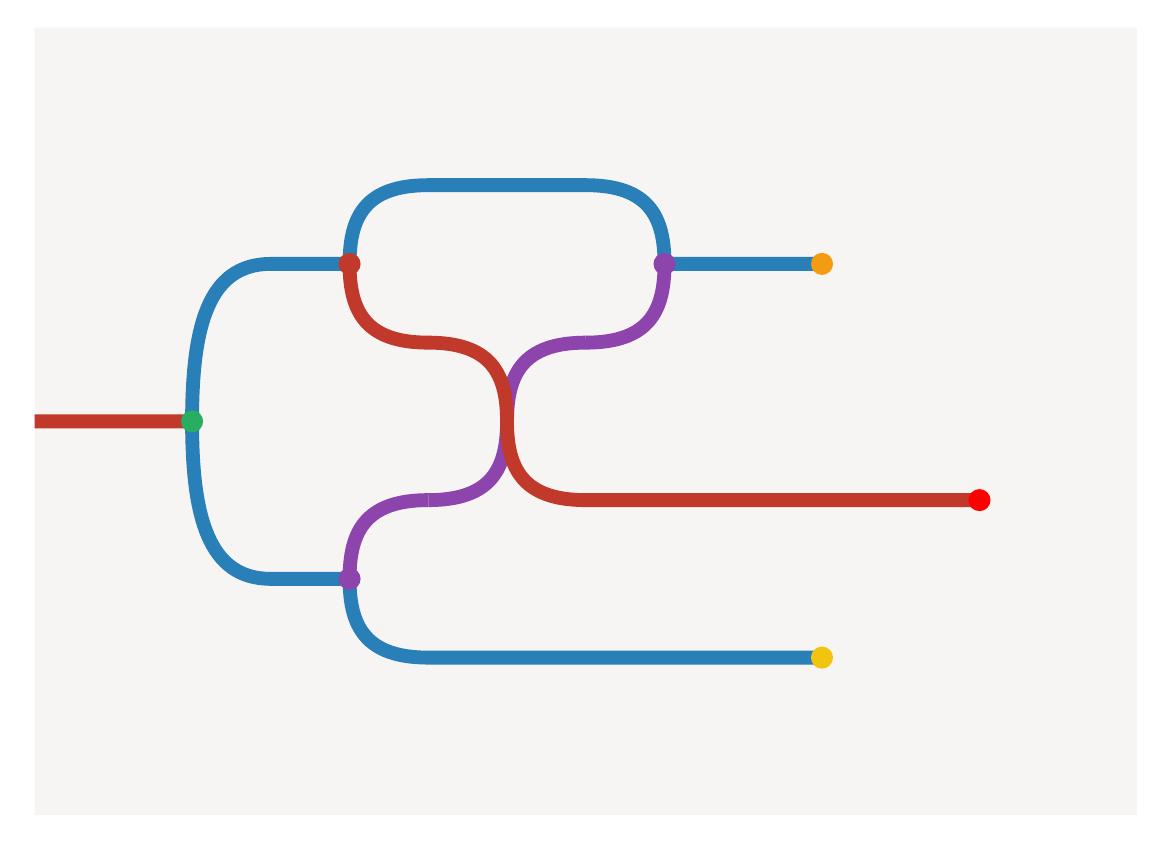
\begin{tikzpicture}
\definecolor{generator-13-5-0-pos}{RGB}{192, 57, 43}
\definecolor{generator-9-4-0-pos}{RGB}{142, 68, 173}
\definecolor{generator-1-4-0-pos}{RGB}{192, 57, 43}
\definecolor{generator-6-5-0-pos}{RGB}{243, 156, 18}
\definecolor{generator-5-5-0-pos}{RGB}{241, 196, 15}
\definecolor{generator-12-5-0-pos}{RGB}{142, 68, 173}
\definecolor{generator-4-5-0-pos}{RGB}{39, 174, 96}
\definecolor{generator-11-5-0-pos}{RGB}{142, 68, 173}
\definecolor{generator-0-0-0-pos}{RGB}{246, 245, 244}
\definecolor{generator-3-5-0-pos}{RGB}{255, 0, 0}
\definecolor{generator-2-4-0-pos}{RGB}{41, 128, 185}
\begin{scope}
% Background surfaces
\fill[generator-0-0-0-pos] (0,-0) -- (0,-10) -- (14,-10) -- (14,-0) -- (0,-0);
% Wire layers
\draw[color=generator-9-4-0-pos, line width=5pt](5,-6) .. controls (5.8,-6) and (6,-5.6) .. (6,-5) .. controls (6,-4.4) and (6.2,-4) .. (7,-4);
\draw[color=generator-1-4-0-pos, line width=5pt](0,-5) -- (2,-5)(4,-3) .. controls (4,-3.6) and (4.2,-4) .. (5,-4) .. controls (5.8,-4) and (6,-4.4) .. (6,-5) .. controls (6,-5.6) and (6.2,-6) .. (7,-6) -- (12,-6);
\draw[color=generator-9-4-0-pos, line width=5pt](4,-7) .. controls (4,-6.4) and (4.2,-6) .. (5,-6)(7,-4) .. controls (7.8,-4) and (8,-3.6) .. (8,-3);
\draw[color=generator-2-4-0-pos, line width=5pt](2,-5) .. controls (2,-3.8) and (2.2,-3) .. (3,-3) -- (4,-3) .. controls (4,-2.4) and (4.2,-2) .. (5,-2) -- (7,-2) .. controls (7.8,-2) and (8,-2.4) .. (8,-3) -- (10,-3)(2,-5) .. controls (2,-6.2) and (2.2,-7) .. (3,-7) -- (4,-7) .. controls (4,-7.6) and (4.2,-8) .. (5,-8) -- (10,-8);
\end{scope}
\fill[generator-4-5-0-pos] (2,-5) circle (0.14);
\fill[generator-13-5-0-pos] (4,-3) circle (0.14);
\fill[generator-12-5-0-pos] (4,-7) circle (0.14);
\fill[generator-11-5-0-pos] (8,-3) circle (0.14);
\fill[generator-6-5-0-pos] (10,-3) circle (0.14);
\fill[generator-5-5-0-pos] (10,-8) circle (0.14);
\fill[generator-3-5-0-pos] (12,-6) circle (0.14);
\end{tikzpicture}
\]
\[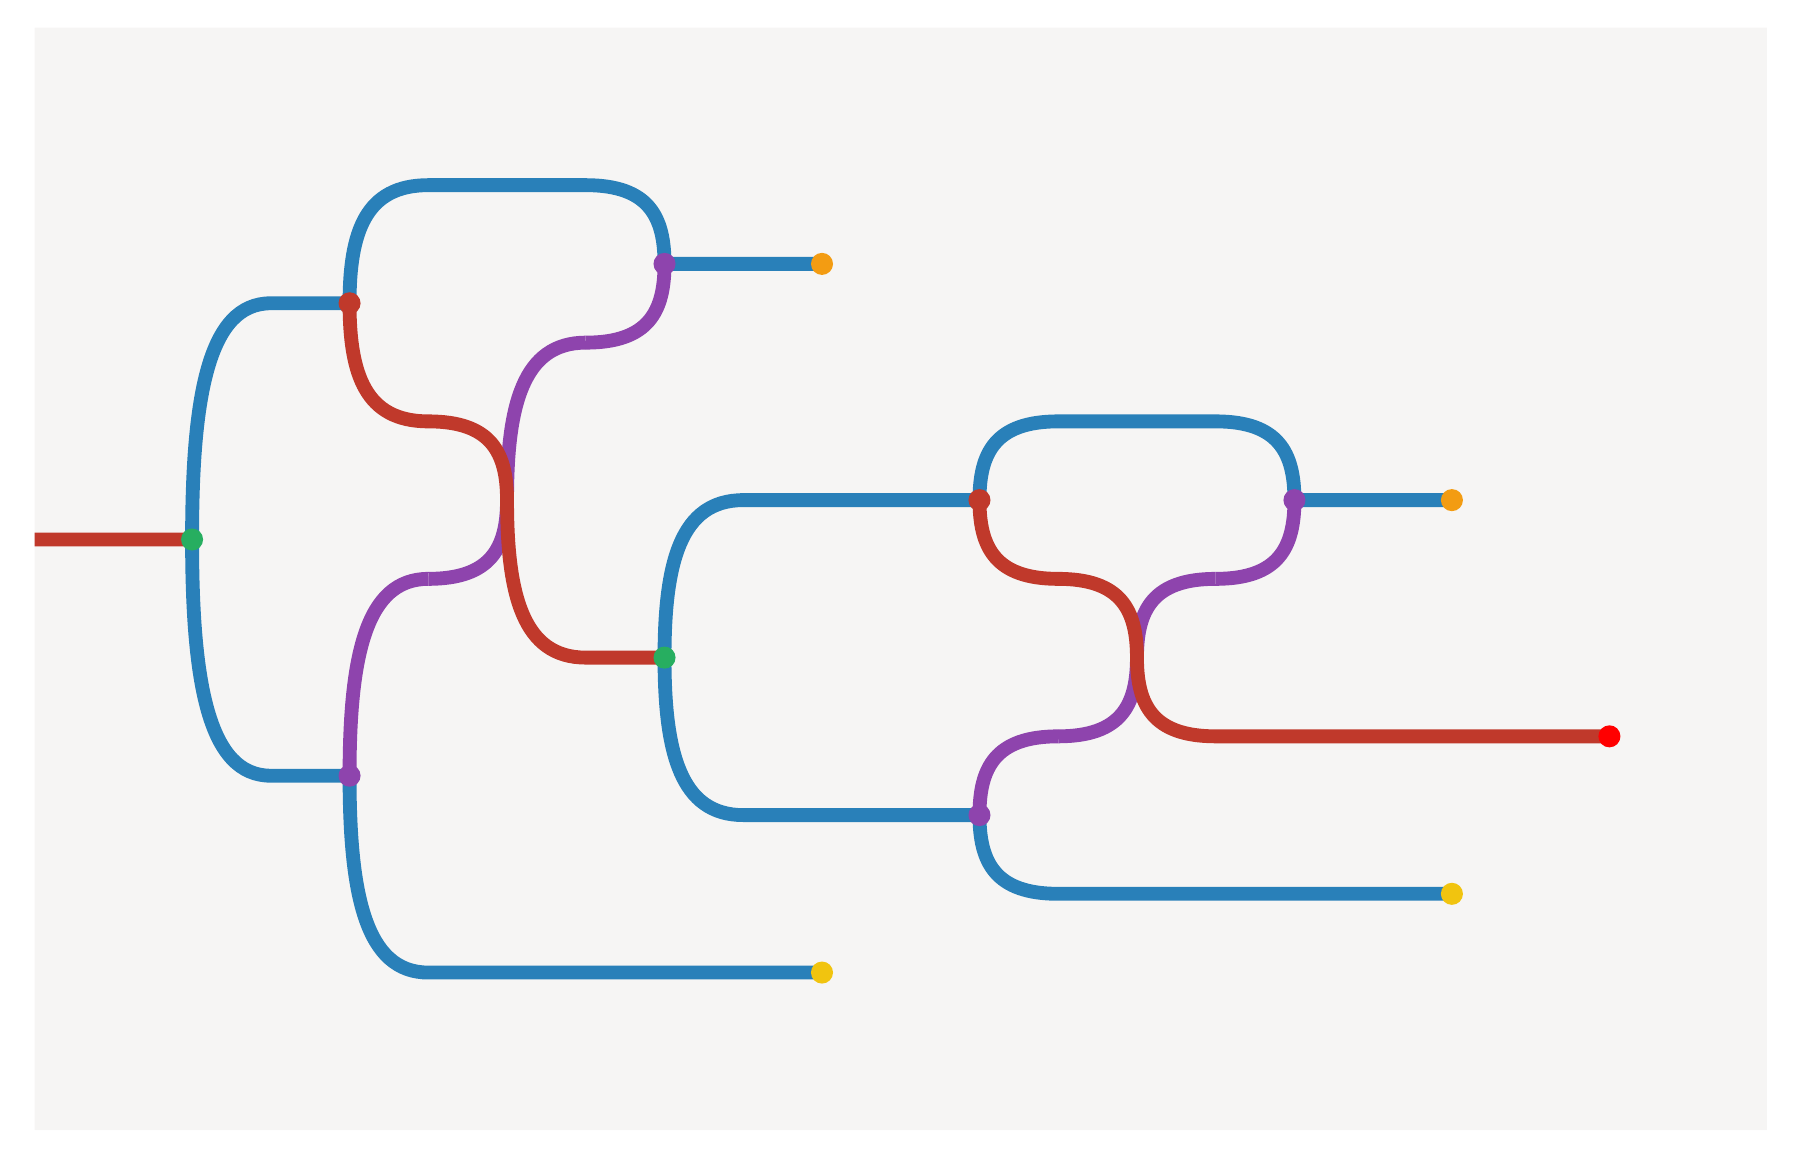
\begin{tikzpicture}
\definecolor{generator-13-5-0-pos}{RGB}{192, 57, 43}
\definecolor{generator-9-4-0-pos}{RGB}{142, 68, 173}
\definecolor{generator-1-4-0-pos}{RGB}{192, 57, 43}
\definecolor{generator-6-5-0-pos}{RGB}{243, 156, 18}
\definecolor{generator-5-5-0-pos}{RGB}{241, 196, 15}
\definecolor{generator-12-5-0-pos}{RGB}{142, 68, 173}
\definecolor{generator-4-5-0-pos}{RGB}{39, 174, 96}
\definecolor{generator-11-5-0-pos}{RGB}{142, 68, 173}
\definecolor{generator-0-0-0-pos}{RGB}{246, 245, 244}
\definecolor{generator-3-5-0-pos}{RGB}{255, 0, 0}
\definecolor{generator-2-4-0-pos}{RGB}{41, 128, 185}
\begin{scope}
% Background surfaces
\fill[generator-0-0-0-pos] (0,-0) -- (0,-14) -- (22,-14) -- (22,-0) -- (0,-0);
% Wire layers
\draw[color=generator-9-4-0-pos, line width=5pt](5,-7) .. controls (5.8,-7) and (6,-6.6) .. (6,-6) .. controls (6,-4.8) and (6.2,-4) .. (7,-4)(13,-9) .. controls (13.8,-9) and (14,-8.6) .. (14,-8) .. controls (14,-7.4) and (14.2,-7) .. (15,-7);
\draw[color=generator-1-4-0-pos, line width=5pt](0,-6.5) -- (2,-6.5)(4,-3.5) .. controls (4,-4.4) and (4.2,-5) .. (5,-5) .. controls (5.8,-5) and (6,-5.4) .. (6,-6) .. controls (6,-7.2) and (6.2,-8) .. (7,-8) -- (8,-8)(12,-6) .. controls (12,-6.6) and (12.2,-7) .. (13,-7) .. controls (13.8,-7) and (14,-7.4) .. (14,-8) .. controls (14,-8.6) and (14.2,-9) .. (15,-9) -- (20,-9);
\draw[color=generator-9-4-0-pos, line width=5pt](4,-9.5) .. controls (4,-8) and (4.2,-7) .. (5,-7)(7,-4) .. controls (7.8,-4) and (8,-3.6) .. (8,-3)(12,-10) .. controls (12,-9.4) and (12.2,-9) .. (13,-9)(15,-7) .. controls (15.8,-7) and (16,-6.6) .. (16,-6);
\draw[color=generator-2-4-0-pos, line width=5pt](2,-6.5) .. controls (2,-4.7) and (2.2,-3.5) .. (3,-3.5) -- (4,-3.5) .. controls (4,-2.6) and (4.2,-2) .. (5,-2) -- (7,-2) .. controls (7.8,-2) and (8,-2.4) .. (8,-3) -- (10,-3)(2,-6.5) .. controls (2,-8.3) and (2.2,-9.5) .. (3,-9.5) -- (4,-9.5) .. controls (4,-11) and (4.2,-12) .. (5,-12) -- (10,-12)(8,-8) .. controls (8,-6.8) and (8.2,-6) .. (9,-6) -- (12,-6) .. controls (12,-5.4) and (12.2,-5) .. (13,-5) -- (15,-5) .. controls (15.8,-5) and (16,-5.4) .. (16,-6) -- (18,-6)(8,-8) .. controls (8,-9.2) and (8.2,-10) .. (9,-10) -- (12,-10) .. controls (12,-10.6) and (12.2,-11) .. (13,-11) -- (18,-11);
\end{scope}
\fill[generator-4-5-0-pos] (2,-6.5) circle (0.14);
\fill[generator-13-5-0-pos] (4,-3.5) circle (0.14);
\fill[generator-12-5-0-pos] (4,-9.5) circle (0.14);
\fill[generator-11-5-0-pos] (8,-3) circle (0.14);
\fill[generator-4-5-0-pos] (8,-8) circle (0.14);
\fill[generator-6-5-0-pos] (10,-3) circle (0.14);
\fill[generator-5-5-0-pos] (10,-12) circle (0.14);
\fill[generator-13-5-0-pos] (12,-6) circle (0.14);
\fill[generator-12-5-0-pos] (12,-10) circle (0.14);
\fill[generator-11-5-0-pos] (16,-6) circle (0.14);
\fill[generator-6-5-0-pos] (18,-6) circle (0.14);
\fill[generator-5-5-0-pos] (18,-11) circle (0.14);
\fill[generator-3-5-0-pos] (20,-9) circle (0.14);
\end{tikzpicture}
\]
\[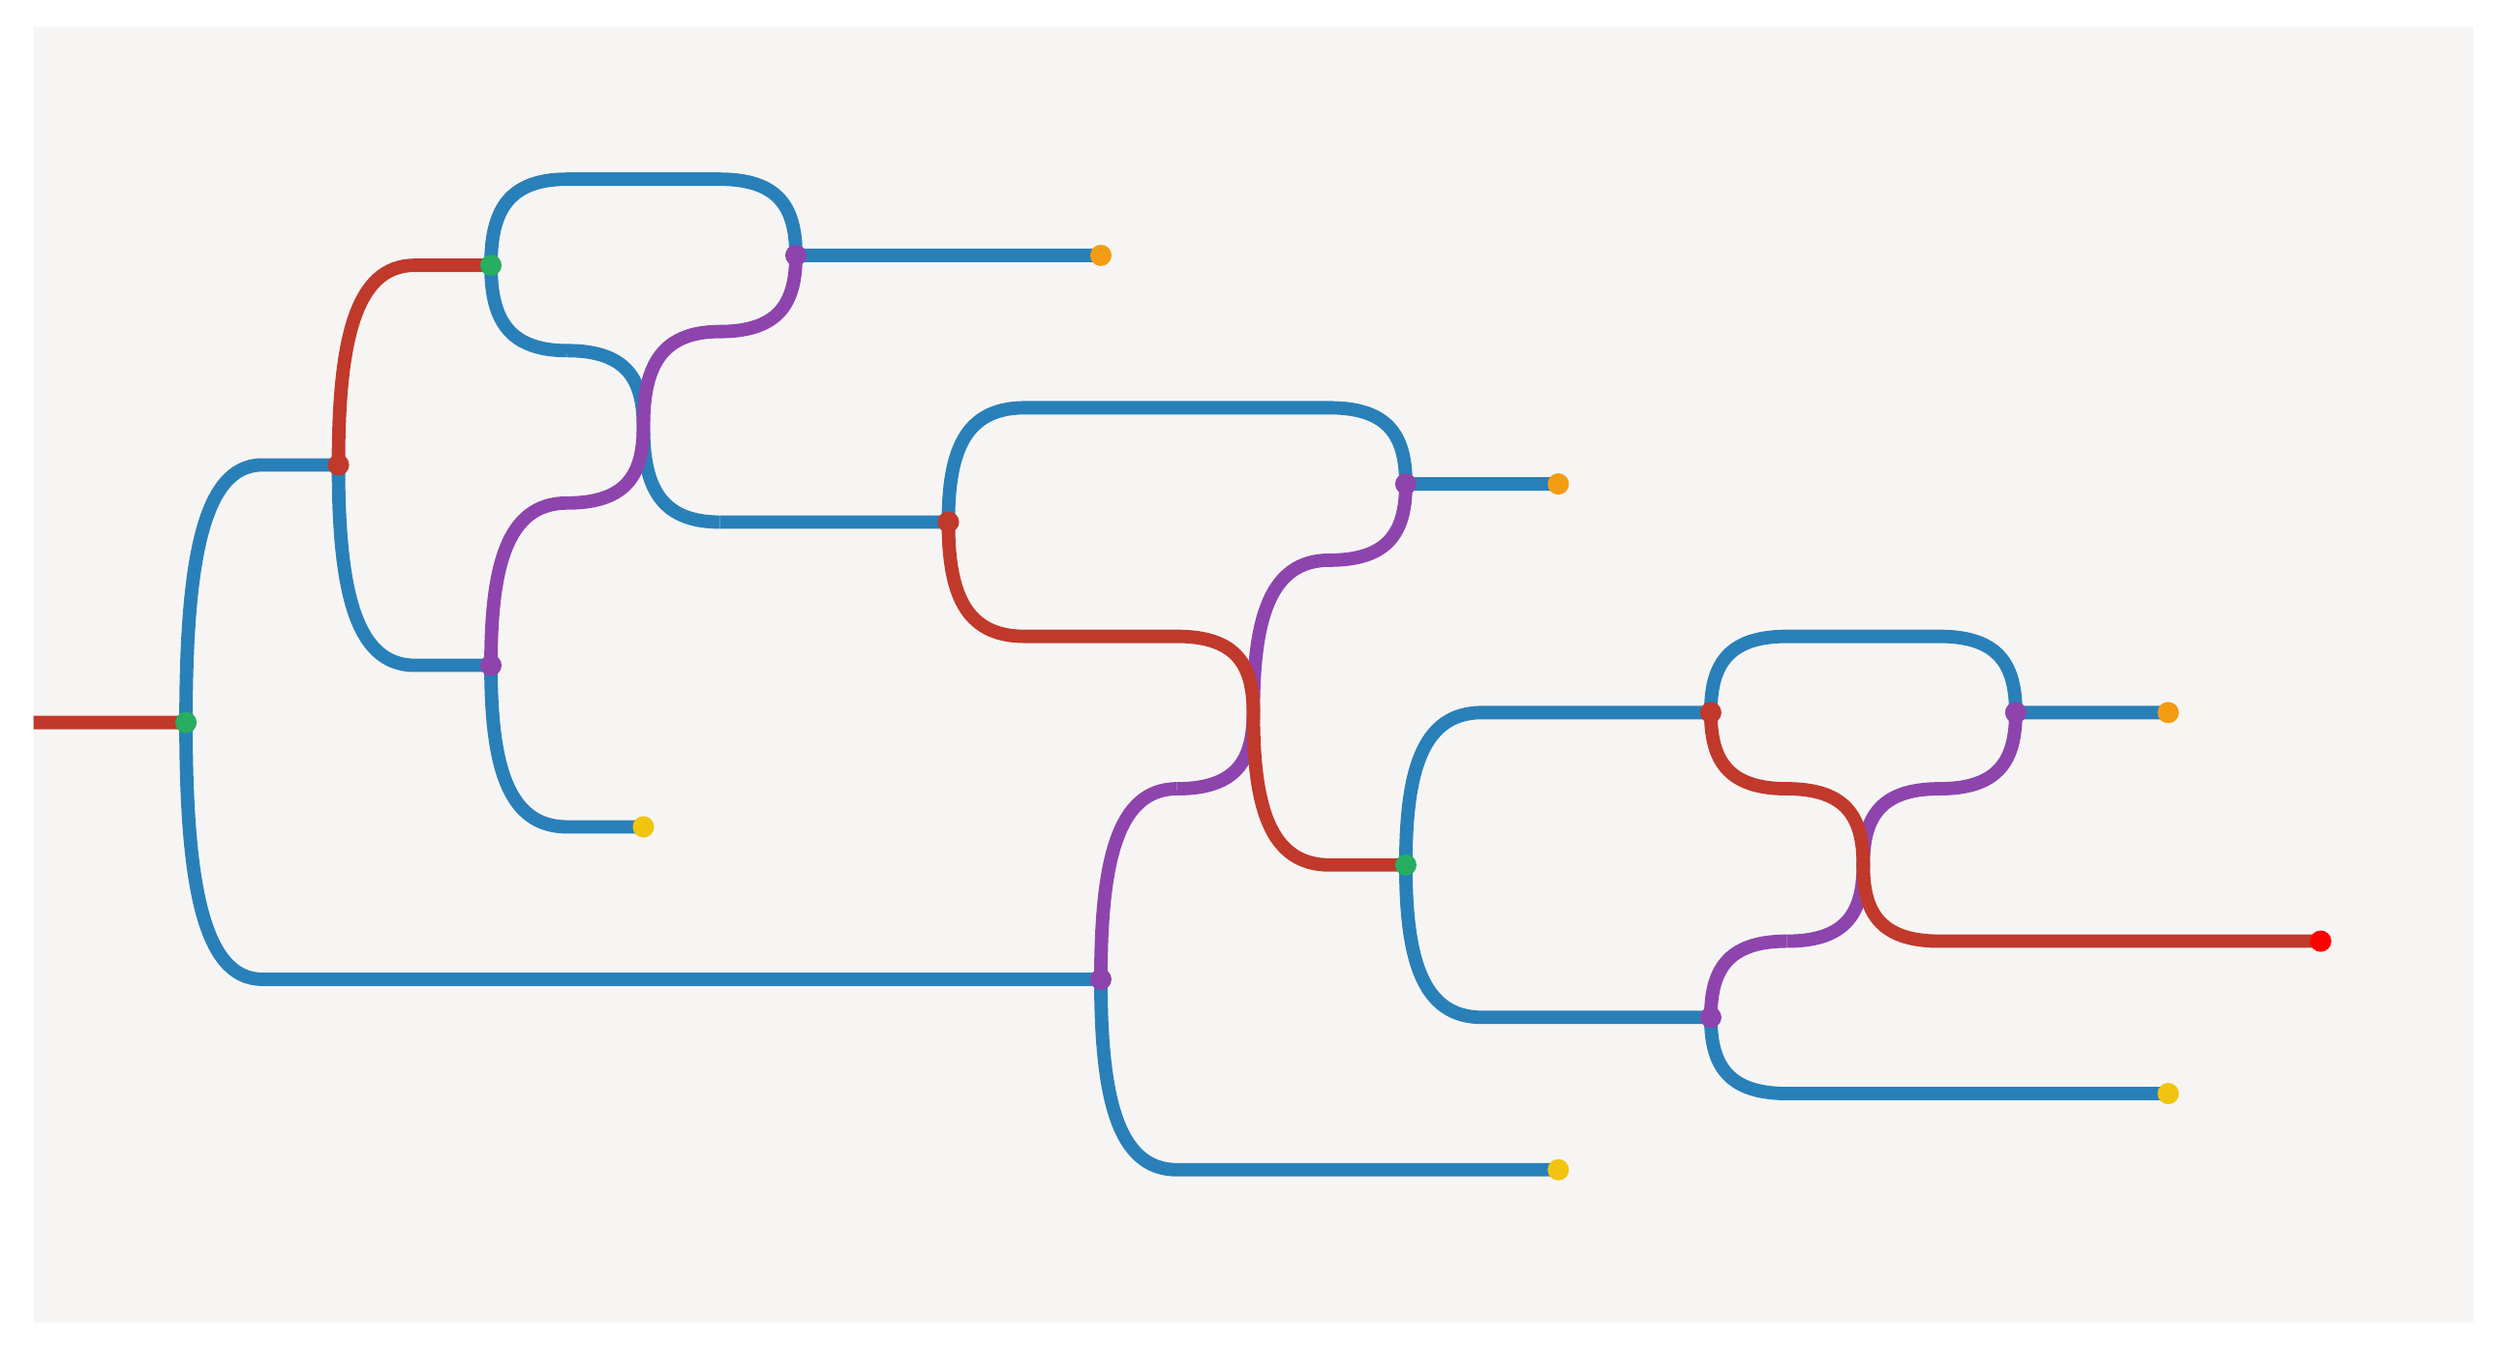
\begin{tikzpicture}
\definecolor{generator-13-5-0-pos}{RGB}{192, 57, 43}
\definecolor{generator-9-4-0-pos}{RGB}{142, 68, 173}
\definecolor{generator-1-4-0-pos}{RGB}{192, 57, 43}
\definecolor{generator-5-5-0-pos}{RGB}{241, 196, 15}
\definecolor{generator-6-5-0-pos}{RGB}{243, 156, 18}
\definecolor{generator-12-5-0-pos}{RGB}{142, 68, 173}
\definecolor{generator-8-5-0-pos}{RGB}{192, 57, 43}
\definecolor{generator-4-5-0-pos}{RGB}{39, 174, 96}
\definecolor{generator-11-5-0-pos}{RGB}{142, 68, 173}
\definecolor{generator-0-0-0-pos}{RGB}{246, 245, 244}
\definecolor{generator-3-5-0-pos}{RGB}{255, 0, 0}
\definecolor{generator-2-4-0-pos}{RGB}{41, 128, 185}
\begin{scope}
% Background surfaces
\fill[generator-0-0-0-pos] (0,-0) -- (0,-17) -- (32,-17) -- (32,-0) -- (0,-0);
% Wire layers
\draw[color=generator-9-4-0-pos, line width=5pt](15,-10) .. controls (15.8,-10) and (16,-9.6) .. (16,-9) .. controls (16,-7.8) and (16.2,-7) .. (17,-7)(23,-12) .. controls (23.8,-12) and (24,-11.6) .. (24,-11) .. controls (24,-10.4) and (24.2,-10) .. (25,-10);
\draw[color=generator-2-4-0-pos, line width=5pt](7,-4.25) .. controls (7.8,-4.25) and (8,-4.65) .. (8,-5.25) .. controls (8,-6) and (8.2,-6.5) .. (9,-6.5);
\draw[color=generator-1-4-0-pos, line width=5pt](0,-9.13) -- (2,-9.13)(4,-5.75) .. controls (4,-4.18) and (4.2,-3.13) .. (5,-3.13) -- (6,-3.13)(12,-6.5) .. controls (12,-7.4) and (12.2,-8) .. (13,-8) -- (15,-8) .. controls (15.8,-8) and (16,-8.4) .. (16,-9) .. controls (16,-10.2) and (16.2,-11) .. (17,-11) -- (18,-11)(22,-9) .. controls (22,-9.6) and (22.2,-10) .. (23,-10) .. controls (23.8,-10) and (24,-10.4) .. (24,-11) .. controls (24,-11.6) and (24.2,-12) .. (25,-12) -- (30,-12);
\draw[color=generator-9-4-0-pos, line width=5pt](6,-8.38) .. controls (6,-7.1) and (6.2,-6.25) .. (7,-6.25) .. controls (7.8,-6.25) and (8,-5.85) .. (8,-5.25) .. controls (8,-4.5) and (8.2,-4) .. (9,-4) .. controls (9.8,-4) and (10,-3.6) .. (10,-3)(14,-12.5) .. controls (14,-11) and (14.2,-10) .. (15,-10)(17,-7) .. controls (17.8,-7) and (18,-6.6) .. (18,-6)(22,-13) .. controls (22,-12.4) and (22.2,-12) .. (23,-12)(25,-10) .. controls (25.8,-10) and (26,-9.6) .. (26,-9);
\draw[color=generator-2-4-0-pos, line width=5pt](2,-9.13) .. controls (2,-7.1) and (2.2,-5.75) .. (3,-5.75) -- (4,-5.75) .. controls (4,-7.33) and (4.2,-8.38) .. (5,-8.38) -- (6,-8.38) .. controls (6,-9.65) and (6.2,-10.5) .. (7,-10.5) -- (8,-10.5)(2,-9.13) .. controls (2,-11.15) and (2.2,-12.5) .. (3,-12.5) -- (14,-12.5) .. controls (14,-14) and (14.2,-15) .. (15,-15) -- (20,-15)(6,-3.13) .. controls (6,-2.45) and (6.2,-2) .. (7,-2) -- (9,-2) .. controls (9.8,-2) and (10,-2.4) .. (10,-3) -- (14,-3)(6,-3.13) .. controls (6,-3.8) and (6.2,-4.25) .. (7,-4.25)(9,-6.5) -- (12,-6.5) .. controls (12,-5.6) and (12.2,-5) .. (13,-5) -- (17,-5) .. controls (17.8,-5) and (18,-5.4) .. (18,-6) -- (20,-6)(18,-11) .. controls (18,-9.8) and (18.2,-9) .. (19,-9) -- (22,-9) .. controls (22,-8.4) and (22.2,-8) .. (23,-8) -- (25,-8) .. controls (25.8,-8) and (26,-8.4) .. (26,-9) -- (28,-9)(18,-11) .. controls (18,-12.2) and (18.2,-13) .. (19,-13) -- (22,-13) .. controls (22,-13.6) and (22.2,-14) .. (23,-14) -- (28,-14);
\end{scope}
\fill[generator-4-5-0-pos] (2,-9.13) circle (0.14);
\fill[generator-8-5-0-pos] (4,-5.75) circle (0.14);
\fill[generator-4-5-0-pos] (6,-3.13) circle (0.14);
\fill[generator-12-5-0-pos] (6,-8.38) circle (0.14);
\fill[generator-5-5-0-pos] (8,-10.5) circle (0.14);
\fill[generator-11-5-0-pos] (10,-3) circle (0.14);
\fill[generator-13-5-0-pos] (12,-6.5) circle (0.14);
\fill[generator-6-5-0-pos] (14,-3) circle (0.14);
\fill[generator-12-5-0-pos] (14,-12.5) circle (0.14);
\fill[generator-11-5-0-pos] (18,-6) circle (0.14);
\fill[generator-4-5-0-pos] (18,-11) circle (0.14);
\fill[generator-6-5-0-pos] (20,-6) circle (0.14);
\fill[generator-5-5-0-pos] (20,-15) circle (0.14);
\fill[generator-13-5-0-pos] (22,-9) circle (0.14);
\fill[generator-12-5-0-pos] (22,-13) circle (0.14);
\fill[generator-11-5-0-pos] (26,-9) circle (0.14);
\fill[generator-6-5-0-pos] (28,-9) circle (0.14);
\fill[generator-5-5-0-pos] (28,-14) circle (0.14);
\fill[generator-3-5-0-pos] (30,-12) circle (0.14);
\end{tikzpicture}
\]

\textbf{N.B.} In practice when using \texttt{homotopy.io} for the symmetric monoidal setting, it is simpler to suspend symmetric monoidal signatures to begin at 4-cells rather than 3-cells. The reason for this is that under- and over-braids still exist in the symmetric monoidal setting, and while sequentially composed braids are homotopically equivalent to the pair of identities, they are not uniquely so, thus these homotopies must be input manually. By beginning at 4-cells (or higher, due to the stabilisation hypothesis []), braid-eliminations are unique up to homotopy and can be performed more easily in the proof assistant.
\end{example}

Now we have enough to spell out full TAGs with local constraints and links as an $n$-categorical signature. To recap briefly, we have seen that we can model the passage from CFGs to TAGs in the $n$-categorical setting, and then how selective and null adjoining rules by specifying endomorphisms on wires as the source of rewrites, and finally that we can model links in the symmetric monoidal setting. Maintaining planarity (which is important for a left-to-right order of terminals for spelling out a language) and modelling obligatory rewrites can be done by requiring that \emph{finished} derivations are precisely those whose only twists are link-wires, and have no sources for obligatory adjoins.

\begin{defn}[Tree Adjoining Grammars with local constraints and links in \texttt{homotopy.io}]

A \emph{Linguistic Tree Adjoining Grammar} is given by the following data:

\[(\mathcal{N}, \mathcal{N}^\downarrow, \mathcal{N}^*, \Sigma, \mathcal{I}, \mathcal{A}, \mathfrak{S} \subseteq \mathcal{P}(\mathcal{A}), \Box, \Diamond, \mathfrak{L} \subseteq \mathcal{N})\]

The initial elements are the same as an elementary tree-adjoining grammar and obey the same constraints. The modifications are:

\begin{itemize}
\item{$\mathcal{I}$ is a nonempty set of \emph{initial} constrained-linked-trees.}
\item{$\mathcal{A}$ is a nonempty set of \emph{auxiliary} constrained-linked-trees.}
\item{$\mathfrak{S}$ is a set of sets of \emph{select} auxiliary trees.}
\item{$\Box, \Diamond$ are fresh symbols. $\Box$ marks \emph{obligatory adjoins}, and $\Diamond$ marks \emph{optional} adjoins.}
\item{$\mathfrak{L}$ is a set permissible \emph{link types} among nonterminals or $\top$.}
\end{itemize}
A \emph{constrained-linked-tree}, or CL-tree, is a pair consisting of:
\begin{itemize}
\item{A tree where each internal node is an element of $\mathcal{N} \times \mathfrak{S} \times \{\Box,\Diamond\} \times \{*, \bar{*}\}$, and each leaf is an element of $\mathcal{N} \times \mathfrak{S} \times \{\Box,\Diamond\} \times \{*, \bar{*}\} \cup \Sigma$. In prose, each label is either a terminal symbol (as a leaf), or otherwise a nonterminal, along with a subset of auxiliary trees that indicates select adjoins (or null-adjoins when the subset is $\varnothing$), a marker indicating whether those adjoins are obligatory or optional, and a marker indicating whether the node is a foot node or not. Observe that there is no need to indicate when a node is a valid target for substitution since that function is subsumed by null adjoining rules.}
\item{
A set of ordered pairs of nodes $(n_1,n_2)$ of the tree such that:
\begin{enumerate}
\item{$n_2$ \emph{c-commands} $n_1$, (i.e., $n_2$ is not an ancestor of $n_1$, and there exists a node $m$ which is the immediate parent node of $n_2$, and an ancestor of $n_1$).}
\item{$n_1$ and $n_2$ share the same type $\mathbf{T} \in \mathcal{N}$ and $\mathbf{T} \in \mathfrak{L}$, or both $n_1,n_2$ are terminals.}
\item{$n_1$ is the parent of terminal symbols, or childless.}
\end{enumerate}
}
\end{itemize}

We spell out how this data becomes an $n$-categorical signature by enumerating cell dimensions:

\begin{enumerate}
\setcounter{enumi}{-1}
\item{A single object $\star$}
\item{None.}
\item{None.}
\item{
	\begin{itemize}
	\item{For each $\mathbf{T} \in \mathcal{N}$, a cell $\mathbf{T}: \mathbf{1}_{\mathbf{1}_\star} \rightarrow \mathbf{1}_{\mathbf{1}_\star}$.}
	\item{$\top: \mathbf{1}_{\mathbf{1}_\star} \rightarrow \mathbf{1}_{\mathbf{1}_\star}$ A wire for terminal symbols.}
	\item{For each $\mathbf{L} \in \mathfrak{L}$, a cell $\mathbf{L} : \mathbf{1}_{\mathbf{1}_\star} \rightarrow \mathbf{1}_{\mathbf{1}_\star}$.}
	\end{itemize}
}
\item{
	We distinguish between \emph{atomic} and \emph{composite} generators at this level. The trees themselves are composites of \emph{atomic} generators. The \emph{atomic} generators are:
	\begin{itemize}
	\item{For each node $n$ that occurs in either $\mathcal{I}$ or $\mathcal{A}$, we populate cells by a case analysis:
	\begin{itemize}
		\item{If $n$ is a terminal $\sigma \in \Sigma$, we create a cell $\sigma: \top \rightarrow \mathbf{1}_{\mathbf{1}_{\mathbf{1}_\star}}$.}
		\item{If $n = (\mathbf{T},\mathbf{S},\dagger,\bar{*})$, we create $\mathbf{S}_\mathbf{T}^\Box: \mathbf{T} \rightarrow \mathbf{T}$ if the node is marked obligatory ($\dagger = \Box$), and a cell $\mathbf{S}_\mathbf{T}^\Diamond: \mathbf{T} \rightarrow \mathbf{T}$ otherwise.}
		\item{If $n = (\mathbf{T},\mathbf{S},\dagger,*)$, it is a foot note, for which we create a cell $\mathbf{S}_\mathbf{T}^\Box: \mathbf{T} \rightarrow \mathbf{1}_{\mathbf{1}_{\mathbf{1}_\star}}$ if the node is marked obligatory ($\dagger = \Box$), and a cell $\mathbf{S}_\mathbf{T}^\Diamond: \mathbf{T} \rightarrow \mathbf{1}_{\mathbf{1}_{\mathbf{1}_\star}}$ otherwise.}
	\end{itemize}
	}
	\item{For each $\mathbf{L} \in \mathfrak{L}$ (which is also a type $\mathbf{T} \in \mathcal{N}$) a pair of cells $\mathbf{T}^\mathbf{L} := \mathbf{T} \rightarrow \mathbf{T} \otimes \mathbf{L}$ and $\mathbf{T}_\mathbf{L} := \mathbf{L} \otimes \mathbf{T} \rightarrow \mathbf{T}$.}
	\item{For each node $p$ of type $\mathbf{T}_p$ in either $\mathcal{I}$ or $\mathcal{A}$ with a nonempty left-to-right list of children $C_p := <c_1,c_2,\cdots c_i, c\dots c_n>$ with types $\mathbf{T}_i$, a branch cell $C_p : \mathbf{T}_p \rightarrow \bigotimes\limits_{i=1}^{n} \mathbf{T}_i$.}
	\end{itemize}
	We represent trees by composite generators, defined recursively. For a given tree $\mathcal{T}$ in either $\mathcal{I}$ or $\mathcal{A}$, we define a composite generator beginning at the root. Where the root node is $p = (\mathbf{T},\mathbf{S},\dagger)$, we begin with the cell $\mathbf{S}_\mathbf{T}^\dagger$. For branches, we compose the branch cell $C_p$ to this cell sequentially. If $p$ has a child $c$ that has a link, we do a case analysis. If that child c-commands the other end of the link we generate the first half of the linking wire by composing $\mathbf{T}^\mathbf{L}$ for the appropriate type $\mathbf{T}$ of the child node. Otherwise the child is c-commanded by a previously generated link, which we braid over and connect using $\mathbf{T}_\mathbf{L}$, again with the appropriate typing for the child. Now we may recurse the procedure for subtrees. If a node has no children, it is a leaf $l = (\mathbf{T},\mathbf{S},\dagger)$ or a terminal symbol. We append a terminal cell $\sigma$ if $l$ is a terminal symbol (thus killing the wire), and otherwise we leave an open $\mathbf{T}$ wire after appending $\mathbf{S}_\mathbf{T}^\dagger$. Altogether this obtains a 3-cell which we denote $\mathcal{T}$, overloading notation; different execution-orders of the above procedure evidently obtain 3-cells equivalent up to homotopy.
}
\item{}
\end{enumerate}

\end{defn}\label{sec:ncat}
\newpage
\newpage

\section{A generative grammar for text circuits}

\subsection{A circuit-growing grammar}

\marginnote{
\begin{defn}[Lexicon]\label{defn:lex}
We define a limited lexicon $\mathcal{L}$ to be a tuple of disjoint finite sets $(\mathbf{N}, \mathbf{V}_1, \mathbf{V}_2, \mathbf{V}_{\texttt{S}}, \mathbf{A}_{\texttt{N}}, \mathbf{A}_{\texttt{V}}, \mathbf{C})$
\end{defn}
}

\marginnote{
Where:
\begin{itemize}
\item $\mathbf{N}$ is a set of \emph{proper nouns}
\item $\mathbf{V}_1$ is a set of \emph{intransitive verbs}
\item $\mathbf{V}_2$ is a set of \emph{transitive verbs}
\item $\mathbf{V}_{\texttt{S}}$ is a set of \emph{sentential-complement verbs}
\item $\mathbf{A}_{\texttt{N}}$ is a set of \emph{adjectives}
\item $\mathbf{A}_{\texttt{V}}$ is a set of \emph{adverbs}
\item $\mathbf{C}$ is a set of \emph{conjunctions}
\end{itemize}
}

\begin{marginfigure}
\centering
\[
\resizebox{\textwidth}{!}{\tikzfig{mushroom/howtoread}}
\]
\caption{\textbf{How to read the diagrams in this section:} we will be making heavy use of pink and purple bubbles as frames to construct circuits. We will depict the bubbles horizontally, as we are permitted to by compact closure, or by reading diagrams with slightly skewed axes.}
\end{marginfigure}

There are many different ways to write a weak $n$-categorical signature that generates circuits. Mostly as an illustration of expressivity, I will provide a signature where the terms "surface" and "deep" structure are taken literally as metaphors; the generative grammar will grow a line of words in syntactic order, and like mushrooms on soil, the circuits will behave as the mycelium underneath the words. It won't be the most efficient way to do it in terms of the number of rules to consider, but it will look nice and we'll be able to reason about it easily.\\

\newthought{Simplifications and limitations}: For now we only consider word types as in Definition \ref{defn:lex}, though we will see how to engineer extensions later. We only deal with propositional statements, without determiners, in only one tense, with no morphological agreement between nouns and their verbs and referring pronouns, and we assume that adverbs, adjectives stack indefinitely and without further order requirements: e.g. \texttt{Alice happily secretly finds red big toy shiny car that he gives to Bob} is a sentence we consider grammatical enough. For now, we consider only the case where adjectives and adverbs appear before their respective noun or verb. Note that all of these limitations apart from the limited lexicon can principle be overcome by the techniques we developed in Section \ref{sec:ncat} for restricted tree-adjoining and links. As a historical remark, generative-transformational grammars fell out of favour linguistically due to the problem of overgeneration: the generation of nonsense or unacceptable sentences in actual language use. We're undergenerating and overgenerating at the same time, but we're also not concerned with empirical capture: we only require a concrete mathematical basis to build interesting things on top of. On a related note, there's zero chance that this particular circuit-growing grammar even comes close to how language is actually produced by humans, and I have no idea whether a generalised graph-rewriting approach is cognitively realistic.

\newthought{Mathematical assumptions}: We work in a dimension where wires behave symmetric monoidally by homotopy, and further assume strong compact closure rewrite rules for all wire-types. Our strategy will be to generate "bubbles" for sentences, within which we can grow circuit structure piecemeal. We will only express the rewrite rules; the generators of lower dimension are implicit. We aim to recover the linear ordering of words in text (essential to any syntax) by traversing the top surface of a chain of bubbles representing sentence structure in text -- this order will be invariant up to compact closed isomorphisms. The diagrammatic consequence of these assumptions is that we will be working with a conservative generalisation of graph-rewriting defined by local rewriting rules. The major distinction is that locality can be redefined up to homotopy, which allows locally-defined rules to operate in what would be a nonlocal fashion in terms of graph neighbourhoods, as in Figure \ref{fig:locality}. The minor distinction is that rewrite rules are sensitive to twists in wires and the radial order in which wires emanate from nodes, though it is easy to see how these distinctions can be circumvented by additional by imposing the equivalent of commutativity relations as bidirectional rewrites. It is worth remarking that one can devise weak n-categorical signatures to simulate turing machines, where output strings are e.g. 0-cells on a selected 1-cell, so rewrite systems of the kind we propose here are almost certainly expressively sufficient for anything; the real benefit is the interpretable geometric intuitions of the diagrams.

\begin{figure}[h!]\label{fig:locality}
\centering
\[
\resizebox{\textwidth}{!}{\tikzfig{mushroom/locality}}
\]
\caption{In this toy example, obtaining the same rewrite that connects the two yellow nodes with a purple wire using only graph-theoretically-local rewrites could potentially require an infinite family of rules for all possible configurations of pink and cyan nodes that separate the yellow, or would otherwise require disturbing other nodes in the rewrite process. In our setting, strong compact closure homotopies handle navigation between different spatial presentations so that a single rewrite rule suffices: the source and target notated by dotted-black circles. Despite the expressive economy and power of finitely presented signatures, we cannot "computationally cheat" graph isomorphism: formally we must supply the compact-closure homotopies as part of the rewrite, absorbed and hidden here by the $\simeq$ notation.}
\end{figure}

\newthought{The plan}: We start with simple sentences that only contain a single intransitive or transitive verb. Then we consider more general sentences. For these two steps, we characterise the expressive capacity of our rules in terms of a context-sensitive grammar that corresponds to the surface structure of the derivations. Then we introduce text structure as lists of sentences with coreferential structure on nouns, along with a mathematical characterisation of coreferential structure and a completeness result of our rules with respect to them. Then we (re)state and prove the text circuit theorem: that the fragment of language we have built with the syntax surjects onto text circuits. Finally we examine how we may model extensions to the expressive capacity of text circuits by introduction of new rewrite rules.

\clearpage

\subsection{Simple sentences}

\marginnote{
\begin{defn}[CSG for simple sentences]\label{dfn:simpCSG}
We may gauge the expressivity of simple sentences with the following context sensitive grammar.
\end{defn}
}

\marginnote{For verbs, adjectives, and modifiers, depicted unsaturated nouns as dotted and saturated with solid black lines, we have:
\[
\resizebox{\marginparwidth}{!}{\tikzfig{mushroom/simpleCFG}}
\]
}

\marginnote{
Adpositions require several helper-generators; we depict for example the beginning of the sequence of derivations that result from appending adpositions to an intransitive verb (the generators are implicit in the derivations):
\[
\resizebox{0.75\marginparwidth}{!}{\tikzfig{mushroom/simpleADP}}
\]
}

\marginnote{
\begin{proposition}\label{prop:simpsent}
Up to labels, the simple-sentence rules yield the same simple sentences as the CSG for simple sentences.
\begin{proof}
By graphical correspondence; viewing nodes on the pink surface as 1-cells, each rewrite rule yields a 2-cell. For example, for the \textcolor{green}{\texttt{IV}}-intro:
\[
\resizebox{0.5\marginparwidth}{!}{\tikzfig{mushroom/simpcorr}}
\]
\end{proof}
\end{proposition}
}

Simple sentences are sentences that only contain a single intransitive or transitive verb. Simple sentences will contain at least one noun, and may optionally contain adjectives, adverbs, and adpositions. The rules for generating simple sentences are as follows:

\[
\resizebox{\textwidth}{!}{\tikzfig{mushroom/simplesentences}}
\]

The $\texttt{N}_\uparrow$-intro rule introduces new unsaturated nouns from the end of a simple sentence. The \textcolor{green}{\texttt{IV}}-intro rule applies when there is precisely one unsaturated noun in the sentence, and the \textcolor{green}{\texttt{TV}}-intro rule applies when there are precisely two. Both verb-introduction rules saturate their respective nouns, which we depict with a black bulb. Adjectives may be introduced immediately preceding saturated nouns, and adverbs may be introduced immediately preceding any kind of verb. The position of adpositions in English is context-sensitive. To capture this, the $\textcolor{blue}{\texttt{ADP}}_{\textcolor{green}{\texttt{V}}}$-tendril rule allows an unsaturated adposition to appear immediately after a verb; a bulb may travel by homotopy to the right, seeking an unsaturated noun. Conversely, the bidirectional $\textcolor{blue}{\texttt{ADP}}_{\texttt{N}}$-tendril rule sends a mycelic tendril to the left, seeking a verb. The two pass-rules allow unsaturated adpositions to swap past saturated nouns and adjectives; note that by construction, neither verbs nor adverbs will appear in a simple sentence to the right of a verb, so unsaturated adpositions will move right until encountering an unsaturated noun. In case it doesn't, the tendril- and pass- rules are bidirectional and reversible.

\clearpage

\subsection{Complex sentences}

Now we consider two refinements; conjunctions, and verbs that take sentential complements. we may have two sentences joined by a conjunction, e.g. \texttt{Alice dances \underline{while} Bob drinks}. We may also have verbs that take a sentential complement rather than a noun phrase, e.g. \texttt{Alice \underline{sees} Bob dance}; these verbs require nouns, which we depict as wires spanning bubbles.

\begin{figure}[h!]\label{fig:sentbestiary}
\centering
\[
\resizebox{\textwidth}{!}{\tikzfig{mushroom/Sbestiary}}
\]
\caption{The dotted-blue wires do not contentfully interact with anything else; they will serve as visual aids for circuit-translation later, to indicate the contents of boxes. They do however indicate a diagrammatic strategy for extensions to accommodate noun phrases, to be explored later.}
\end{figure}

\marginnote{
\begin{defn}[Sentence structure]\label{dfn:sentCSG}
A sentence can be:
\begin{itemize}
\item a simple sentence, which...
\item ... may generate unsaturated nouns from the right.
\item a pair of sentences with a conjunction in between.
\item (if there is a single unsaturated noun) a sentence with a sentential-complement verb that scopes over a sentence.
\end{itemize}
As a CSG, these considerations are respectively depicted as:
\end{defn}
\[
\resizebox{\marginparwidth}{!}{\tikzfig{mushroom/complexsentenceCSG}}
\]
}

\marginnote{
\begin{proposition}\label{prop:compsent}
Up to labels, the rules so far yield the same sentences as the combined CSG of Definitions \ref{dfn:simpCSG} and \ref{dfn:sentCSG}.
\begin{proof}
Same correspondence as Proposition \ref{prop:simpsent}, ignoring the dotted-blue guards.
\end{proof}
\end{proposition}
}

\begin{figure}[h!]\label{fig:soberA}
\centering
\[
\resizebox{\textwidth}{!}{\tikzfig{mushroom/soberA}}
\]
\caption{
\begin{example}[\texttt{sober} $\alpha$ \texttt{sees drunk} $\beta$ \texttt{clumsily dance.}]
Now we can see our rewrites in action for sentences. As a matter of convention -- reflected in how the various pass- rules do not interact with labels -- we assume that labelling occurs after all of the words are saturated. We have still not introduced rules for labelling nouns: we delay their consideration until we have settled coreferential structure. For now they are labelled informally with greeks.
\end{example}
}
\end{figure}

\begin{figure}[h!]\label{fig:Alaughs}
\centering
\[
\resizebox{\textwidth}{!}{\tikzfig{mushroom/Alaughs}}
\]
\caption{
\begin{example}[$\alpha$ \texttt{laughs at} $\beta$]
Adpositions form by first sprouting and connecting tendrils under the surface. Because the tendril- and pass- rules are bidirectional, extraneous tendrils can always be retracted, and failed attempts for verbs to find an adpositional unsaturated noun argument can be undone. Though this seems computationally wasteful, it is commonplace in generative grammars to have the grammar overgenerate and later define the set of sentences by restriction, which is reasonable so long as computing the restriction is not computationally hard. In our case, observe that once a verb has been introduced and its argument nouns have been saturated, only the introduction of adpositions can saturate additionally introduced unsaturated nouns. Therefore we may define the finished sentences of the circuit-growing grammar to be those that e.g. contain no unsaturated nodes on the surface, which is a very plausible linear-time check by traversing the surface.
\end{example}
}
\end{figure}

\clearpage

\subsection{Text structure and noun-coreference}

\begin{figure}[h!]
\centering
\[
\tikzfig{mushroom/sintro}
\]
\caption{Only considering words, text is just a list of sentences. However, for our purposes, text additionally has \emph{coreferential structure}. Ideally, we would like to connect "the same noun" from distinct sentences as we would circuits.}
\end{figure}

\begin{figure}[h!]
\centering
\[
\tikzfig{mushroom/circuitplan}
\]
\caption{We choose the convention of connecting from left-to-right and from bottom-to-top, so that we might read circuits as we would text: the components corresponding to words will be arranged left-to-right and top-to-bottom. Connecting nouns across distinct sentences presents no issue, but a complication arises when connecting nouns within the same sentence as with reflexive pronouns e.g. \texttt{Alice likes herself}.}
\end{figure}

\begin{figure}[h!]\label{fig:reflcomp}
\centering
\[
\tikzfig{mushroom/reflcomplication}
\]
\caption{Reflexive coreference would violate of the processivity condition of string diagrams for symmetric monoidal categories. Not all symmetric monoidal categories possess the appropriate structure to interpret such reflexive pronouns, but there exist interpretative options. From left to right in roughly decreasing stringency, compact closed categories are the most direct solution. More weakly, traced symmetric monoidal categories also suffice. If there are no traces, so long as the noun wire possesses a monoid and comonoid, a convolution works. If all else fails, one can just specify a new gate. We will define coreference structure to exclude such reflexive coreference and revisit the issue as an extension.}
\end{figure}

\newpage

Now we will deal with coreferential structure and noun-labels.
\begin{fullwidth}
\[
\resizebox{1.5\textwidth}{!}{\tikzfig{mushroom/nounbestiary_newnew}}
\]
\end{fullwidth}

The linked-\texttt{N}-intro rules introduce a new unsaturated noun in the next sentence that coreferences the noun in the previous sentence that generated it. The \texttt{N}-shift rules allow any unsaturated noun to move into the next sentence. For both of the previous rules, the $\beta$ variant handles the case where the next sentence is related to the first by a conjunction. Observe that nouns with a forward coreference have two dotted-black wires leaving the root of their wires, which distinguishes them from nouns that only have a backward coreference or no coreference at all, which only have a single dotted-black wire leaving the root of their wire.\\

The \texttt{N}-swap rule variants allow a unsaturated noun with no forward coreferences to swap places with any unsaturated noun that immediately succeeds it.\\

\begin{figure}[h!]\label{fig:nounkinds}
\centering
\[
\resizebox{\textwidth}{!}{\tikzfig{mushroom/nounkinds}}
\]
\caption{At this point, it is worth establishing some terminology about the kinds of unsaturated nouns we have in play. The kinds of nouns are distinguished by their tails. \emph{Lonely} nouns have no coreferences, their tails connect to nothing. \emph{Head} nouns have a forward coreference in text; they have two tails, one that connects to nothing and the other to a noun later in text. \emph{Middle} nouns have a forward and backward coreference; they have two tails, one that connects to a noun in some preceding sentence, and one that connects forward to a noun in a succeeding sentence. \emph{Foot} nouns only have a backward coreference; they have a single tail connecting to a noun in some preceding sentence.}
\end{figure}

\begin{proposition}\label{prop:linkedlist}
The unsaturated noun kinds listed in Figure \ref{fig:nounkinds} are exhaustive, hence nouns that share a coreference are organised as a diagrammatic linked-list.
\begin{proof}
The \texttt{N}-intro rule creates lonely nouns. Head nouns can only be created by the linked-\texttt{N}-intro applied to a lonely noun. Any new noun created by linked-\texttt{N}-intro is a foot noun. The linked-\texttt{N}-intro rule turns foot nouns into middle nouns. These two intro- rules are the only ones that introduce unsaturated nouns, so it remains to demonstrate that no other rules can introduce noun-kinds that fall outside our taxonomy. The \texttt{N}-shift rule changes relative position of either a lonely or foot noun but cannot change its kind. The \texttt{N}-swap rule may start with either a lonely or foot noun on the left and either a head or middle noun on the right, but the outcome of the rule cannot change the starting kinds as tail-arity is conserved.
\end{proof}
\end{proposition}

\begin{proposition}
Let the \emph{population} of unsaturated nouns in a diagram be the multiset of kinds with multiplicity of their occurence. The \texttt{N}-shift and \texttt{N}-swap rules keep the population invariant.
\begin{proof}
By the end of the argument in Proposition \ref{prop:linkedlist}, conservation of tail-arities by these two local rewrites cannot affect the population.
\end{proof}
\end{proposition}



The link-label rule is a (finite) family of rules parameterised by the nouns in the lexicon

\marginnote{
We require a definition of coreference structure in order verify that our rewrite rules are complete with respect to them. One reasonable constraint on coreference in text is that coreference always goes backwards. One way to express this constraint mathematically is the following:
\begin{defn}[Coreference structure]
In a text with $K \in \mathbb{N}$ distinct nouns and their coreferents, the linear order of noun+referents in a text corresponds to a list of positive integers that:
\begin{enumerate}
\item Starts with 1
\item Contains every $k \in [1\cdots K]$
\item For all $k \in [1 \cdots K]$, the head of the list up to the first occurence of $k$ contains all $j < k$.
\end{enumerate}
\end{defn}
}

\marginnote{
\begin{proposition}
The noun-introduction and manipulation rules are expressively complete with respect to coreference structure.
\begin{proof}

\end{proof}
\end{proposition}
}

\newpage

Nouns require verbs in order to be saturated. From left-to-right; if there is precisely one unlabelled noun, we may introduce an unlabelled intransitive verb and saturate the noun so that it is now ready to grow a label; or if there are two unlabelled nouns, we may introduce an unlabelled transitive verb on the surface and saturate the two nouns that will be subject and object; and verbs may be labelled.
\[
\tikzfig{mushroom/simpbestiary}
\]

\subsection{Modifiers}

Modifiers are optional parts of sentences that modify (and hence depend on there being) nouns and verbs. We consider adjectives, adverbs, and adpositions. From left to right; we allow adjectives to sprout immediately before a saturated noun, and we allow adverbs to sprout immediately before any verb.

\[
\tikzfig{mushroom/adjadv}
\]

Adpositions modify verbs by tying in an additional noun argument; e.g. while \texttt{runs} is intransitive, \texttt{runs towards} behaves as a transitive verb. Some more advanced technology is required to place adpositions and their thematic nouns in the correct linear order on the surface. In the left column; an adposition tendril can sprout from a verb via an unsaturated adposition, seeking an unsaturated noun to the right; an unsaturated noun can sprout an tendril seeking a verb to connect to on the left. Both of these rewrites are bidirectional, as tendrils might attempt connection but fail, and so be retracted. In the centre, when an unsaturated adposition and its tendril find an unsaturated noun, they may connect, saturating the adposition so that it is ready to label. In the right column; an unsaturated adposition may move past a saturated noun in the same sentence, which allows multiple adpositions for the same verb; finally, a saturated adposition can be labelled.

\[
\tikzfig{mushroom/adpbestiary}
\]

\subsection{Rewriting to circuit-form}

\newthought{Resolving references}

\[
\tikzfig{mushroom/pronbestiary}
\]

\[
\tikzfig{mushroom/pronres}
\]

\newthought{Connecting circuits}

\newpage
\subsection{Putting it all together}

\begin{figure}[h!]
\centering
\[
\resizebox{\textwidth}{!}{\tikzfig{mushroom/bigex1}}
\]
\caption{Starting from the initial sentence bubble, we generate a new sentence, introduce some nouns and an SCV, and then we connect our references at the bottom.}
\end{figure}

\begin{figure}[h!]
\centering
\[
\resizebox{\textwidth}{!}{\tikzfig{mushroom/bigex2}}
\]
\caption{Then we introduce intransitive verbs to saturate nouns, and we may also sprout some modifying adjectives and adverbs.}
\end{figure}

\begin{figure}[h!]
\centering
\[
\resizebox{\textwidth}{!}{\tikzfig{mushroom/bigex3}}
\]
\caption{For the remaining unsaturated noun, we use the adposition introduction rules to sprout tendrils off of the other verb in the bubble, and connect.}
\end{figure}

\begin{figure}[h!]
\centering
\[
\resizebox{\textwidth}{!}{\tikzfig{mushroom/bigex4}}
\]
\caption{All of the non-noun words may now be labelled.}
\end{figure}

\begin{figure}[h!]
\centering
\[
\resizebox{\textwidth}{!}{\tikzfig{mushroom/bigex5}}
\]
\caption{To begin assigning nouns, observe that by compact closure of the bubble boundaries, we can deform the diagram to obtain suitable forms for our local rewrite rules for link-generation at the bottom.}
\end{figure}

\begin{figure}[h!]
\centering
\[
\resizebox{\textwidth}{!}{\tikzfig{mushroom/bigex6}}
\]
\caption{Now we can introduce our noun labels and linearise our link structure.}
\end{figure}

\begin{figure}[h!]
\centering
\[
\resizebox{\textwidth}{!}{\tikzfig{mushroom/bigex7}}
\]
\caption{Once the link structure is linearised, we can undo the deformation, and propagate links to the surface.}
\end{figure}

\begin{figure}[h!]
\centering
\[
\resizebox{\textwidth}{!}{\tikzfig{mushroom/bigex8}}
\]
\caption{The bubbles may be rearranged to respect circuit-form, such that the propagation of noun labels to the surface traces out the wires of the end circuit.}
\end{figure}

\clearpage
\newpage
\subsection{Extensions I: relative and reflexive pronouns}

\newthought{Subject relative pronouns}

\begin{example}

\end{example}

\newthought{Object relative pronouns}

\begin{example}

\end{example}

\newthought{Reflexive pronouns}

\begin{example}

\end{example}

\subsection{Extensions II: grammar equations}

\newthought{Attributive vs. predicative modifiers}

\begin{example}

\end{example}

\newthought{Copulas}

\begin{example}

\end{example}

\newthought{Possessive pronouns}

\begin{example}

\end{example}

\subsection{Extensions III: higher-order modifiers}

\newthought{Intensifiers}

\begin{example}

\end{example}

\newthought{Comparatives}

\begin{example}

\end{example}

\subsection{Equivalence to internal wirings}

\subsection{Text circuit theorem}

\subsection{Related work}
\newpage
\section{Text circuits: details, demos, developments}\label{sec:circs}

\marginnote{An example from Task 1, "single supporting fact", is:\\
\[\texttt{Mary went to the bathroom.}\]
\[\texttt{John moved to the hallway.}\]
\[\texttt{Mary travelled to the office.}\]
\[\texttt{\textcolor{blue}{(Query:) Where is Mary?}}\]
\[\texttt{(Answer:) office.}\]
Translating the setup of each task into a circuit of neural nets-to-be-learnt, and queries into appropriately typed measurements-to-be-learnt, each bAbi task becomes a training condition in the form of a process-theoretic equation to be satisfied: the depicted composite process ought to be equal to the \texttt{office} state:
\[
\resizebox{0.4\textwidth}{!}{\tikzfig{textcirc/babiex}}
\]
}

This section covers some practical developments, conventions, references for technical details of text circuits. The most striking demonstration to date is that circuits are defined over a large enough fragment of language to \emph{leverage} several bAbi tasks \bR CITE \e, which are a family of 20 general-reasoning text tasks -- the italicised choice of wording will be elaborated shortly. Each family of tasks consists of tuples of text in simple sentences concluded by a question, along with an answer. It was initially believed that world models were required for the solution of these tasks, but they have been solved using transformer architectures \bR CITE \e. While there is no improvement in capabilities by solving bAbi using text circuits, the bAbi tasks have been used as a dataset to learn word gates from data, in a conceptually compliant and compositional manner, detailed in the margin. Surprisingly, despite the low-data, low-compute regime, the tasks for which the current theory has the expressive capacity to cover are solved better by text circuits than by LSTMs; a proof-of-concept that with the aid of appropriate mathematics, not only might fundamental linguistic considerations help rather than hinder NLP, but also that explainability and capability are not mutually exclusive. Experimental details are elaborated in a forthcoming report \bR CITE \e. While there are expressivity constraints contingent on theoretical development, this price buys a good amount of flexibility within the theoretically established domain: text circuits leave room for both learning-from-data and "hand-coded" logical constraints expressed process-theoretically, and naturally accommodate previously computed vector embeddings of words.\\

In practice, the process of obtaining transparently computable text goes through two phases. First, one has to obtain text circuits from text, which is conceptually simple: typelogical parsers for sentences can be modified to produce circuit-components rather than trees, and a separate pronomial resolution module dictates symmetric monoidal compositionality; details are in the same forthcoming report \bR CITE \e. Second, one implements the text circuits on a computer. On quantum computers, boxes are modelled as quantum combs \bR CITE \e. On classical computers, boxes are sandwiches of generic vector-manipulation neural nets, and boxes with 'dot dot dot' typing are interpreted as families of processes, which can be factored for instance as a pair of content-carrying gates along with a monoid+comonoid convolution to accommodate multiplicity of wires; an example of this interpretation of families of processes is the use of an aggregation monoid in graph neural network \bR CITE \e. The theoretical-to-practical upshot of text circuits when compared to DisCoCat is that the full gamut of compositional techniques, variations, and implementation substrates of symmetric monoidal categories may be used for modelling, compared to the restrictions inherent in hypergraph and strongly compact closed categories.\\

In terms of underpinning mathematical theory, the `dot dot dot' notation within boxes that indicates related families of morphisms is graphically formal \citep{wilson_string_2022}, and interpretations of such boxes were earlier formalised in \citep{merry_reasoning_2014,quick_-logic_2015,zamdzhiev_rewriting_2017}. The two forms of interacting composition, one symmetric monoidal and the other by nesting is elsewhere called \emph{produoidal}, and the reader is referred to \bR CITE \e for formal treatment and a coherence theorem. Boxes with holes may be interpreted in several different ways. Firstly, boxes may be considered syntactic sugar for higher-order processes in monoidal closed categories, and boxes are diagrammatically preferable to combs in this regard, since the latter admits a typing pathology where two mutually facing combs interlock. Secondly, boxes need not be decomposable as processes native to the base category, admitting for instance an interpretation as elementwise inversion in linear maps, which specialises in the case of \textbf{Rel} (viewed as \textbf{Vect} over the boolean ring) to negation-by-complement. In some sense, none of these formalities really matter, on the view that text circuits are algebraic jazz for computing with text, where facets are open to interpretation and modification. What follows are brief sketches of avenues for extensions of the theory.

\subsection{Avenues I: syncategorematicity as distributivity}

A useful heuristic for the application of text diagrams is to treat individual text circuits as analogous to propositional contents, and certain logical or temporal connectives as structural operations upon circuits -- rewrites -- that must be applied in order to obtain a purely propositional format. In other words, logical or structural words are to be treated as circuit-manipulation instructions to be executed in order to obtain a circuit, in the same way that $1 + 1$ is only an integer expression once addition has been evaluated. It is suggested here that the $n$-categorical setting is a suitably rich rewriting system to accommodate such rewrites.

\begin{figure}[h!]
\centering
\[\resizebox{\textwidth}{!}{\tikzfig{mushroom/ABdrink}}\]
\caption{
\begin{example}[\textbf{Syncategorematicity I}]
\[\texttt{Alice \underline{and} Bob drink}\]
\end{example}
\emph{Syncategorematic} words are roughly those that have contextually-dependent semantics. Their dependency is usually predicated on the grammatical type of their arguments. In our terms, since we consider the semantics of text circuits to be underpinned by monoidal functors that reify the circuits in a target category, syncategorematic words such as \texttt{and} may be treated as distributive laws. Here \texttt{and} occurs as a conjunction of nouns and is eliminated by distributive-law rewrites within the deep structure of the text diagram \emph{before translation into circuits}. Note that what is meant by \emph{distributive} here is, in string-diagrammatic terms, precisely the same as that in algebra, for expressions such as $a \times (b + c) = (a \times b) + (a \times c)$. A new copy-node for verb labels that has rewrites for all verbs facilitates distribution, and the deep \texttt{and} nodes come in a tensor-dentensor pair analogous to those for nonstrict string diagrams \bR CITE \e. Sources of rewrites are outlined in dashed boxes.
}
\end{figure}
\clearpage
\newpage


\begin{figure}[h!]
\centering
\[\resizebox{\textwidth}{!}{\tikzfig{mushroom/Bdrinksmoke}}\]
\caption{
\begin{example}[\textbf{Syncategorematicity II}]
\[\texttt{Bob drinks \underline{and} smokes}\]
\end{example}
In this example, the same word \texttt{and} is a conjunction of verbs. In this case we choose to interpret the conjunction of verbs as sequential composition, so there is no need for a corresponding detensor for the \texttt{and} of verbs.
}
\end{figure}

\begin{figure}[h!]
\centering
\[\resizebox{\textwidth}{!}{\tikzfig{mushroom/respectively}}\]
\caption{
\begin{example}[\textbf{Coordination}]
\[\texttt{Alice \underline{and} Bob drink beer \underline{and} wine \underline{respectively}}\]
\end{example}
We stand to win in terms of conceptual economy for modelling; more complex phenomena of text structure such as coordination appear to be resolvable in the same framework of distributivity-law rewrites.
}
\end{figure}


\subsection{Avenues II: determiners and quantifiers in context}

Extending the reach of text circuits to determiners, quantifiers, and conditionals appears to require a contextual diagram or process theory in which to evaluate and enforce constraints upon the purely syntactic content of text circuits. The broad strategy sketched here rests upon three tactics. First, as in the neural approach to bAbi, word-gates are considered to be paired with measurement-processes that return an analog of truth values, the latter of which may be generic tests for adjectives as static predicates or verbs as dynamic predicates. The pairing of gates with measurements follows the philosophy of update structures, introduced in Section \bR REF \e and elaborated in more detail in \bR CITE \e. The truth-measurements allow conditionals to be expressed as either circuit-rewrites or constraints on truth-measurements, the latter which are in turn interpretable as loss-functions in the process of training gates. Second, we model context as the rest of the text circuit, which is a modifiably finite model. Third, we suppose we have a way to record and relate alternative circuits. These tactics appear sufficient for a first pass. Determiners may be considered to be context-sensitive connectivity. Universal quantifiers may be analysed in particular finitary contexts as conditionals and constraints on truth-conditional measurements. Existential quantifiers evaluated in the finitary case yield alternative circuits.

\begin{figure}[h!]
\centering
\[\resizebox{\textwidth}{!}{\tikzfig{mushroom/thebeer1}}\]
\caption{
\begin{example}[\textbf{Determiners I}]
\[\texttt{Bob drinks \underline{the} beer} \text{ (among drinks)}\]
\end{example}
Here, \texttt{drinks} is considered transitive and \texttt{the beer} a nesting box for \texttt{drinks} that reaches over to contextual wires representing a selection of beverages. In this case (relying on the implicit uniqueness of \texttt{the}), a series of \texttt{beer?} tests may be computed, and the best match chosen as the resulting argument for \texttt{drinks}.
}
\end{figure}

\begin{figure}[h!]
\centering
\[\resizebox{\textwidth}{!}{\tikzfig{mushroom/thebeer2}}\]
\caption{
\begin{example}[\textbf{Determiners II}]\label{ex:beer2}
\[\texttt{Bob drinks \underline{a} beer} \text{ (among drinks)}\]
\end{example}
We take the logical (and pragmatic) reading of \texttt{a} as $\exists ! x: \texttt{beer?}(x) \wedge \texttt{drinks?}(\texttt{Bob},x)$. Subject to having a method to hold onto alternatives -- in essence an inquisitive semantics approach -- we may create alternative circuits for each successful \texttt{beer?} test.
}
\end{figure}

\clearpage
\newpage

\begin{figure}[h!]
\centering
\[\resizebox{\textwidth}{!}{\tikzfig{mushroom/thebeer3}}\]
\caption{
\begin{example}[\textbf{Determiners III}]
\[\texttt{Bob drinks \underline{a} beer} \text{ (that we didn't know about)}\]
\end{example}
When there are no beers in context, the same statement takes on a dynamic reading: it constitutes the introduction of a beer into discourse. In terms of text circuits, this amounts to introducing a novel beer-state and beer-wire. Determining an appropriate setting to accommodate "arbitrary" vs. "concrete" beers (c.f. Fine's arbitrary objects \bR CITE \e) requires further research and experimentation, but preliminarily it is known that density matrices are capable of modelling semantic entailment \bR CITE \e, at the computational cost of adopting the kronecker product. This diagram doesn't typecheck, but note that it doesn't have to, because our strategy for evaluation of determiners treats circuits as syntactic objects to be manipulated.
}
\end{figure}

\begin{figure}[h!]
\centering
\[\resizebox{\textwidth}{!}{\tikzfig{mushroom/thebeer4}}\]
\caption{
\begin{example}[\textbf{Quantifiers I}]
\[\texttt{Bob drinks \underline{all the beers}} \text{ (in context)}\]
\end{example}
In a finitary context, drinking \texttt{all the beers} amounts to applying the distributivity of \texttt{and} iteratively in that context. In this case, \texttt{all the beers} is treated as a reference-in-context to \texttt{Hells} and \texttt{Duvel}. In the same manner, existential quantifiers in finite contexts can be treated as finitary disjunctions, which is handled by creating alternative circuits, as in Example \ref{ex:beer2}
}
\end{figure}

\clearpage
\newpage

\begin{figure}[h!]
\centering
\[\resizebox{\textwidth}{!}{\tikzfig{mushroom/thebeer5}}\]
\caption{
\begin{example}[\textbf{Quantifiers II}]
\[\texttt{Bob drinks \underline{all} beers} \text{ (generic)}\]
\end{example}
Without the determiner \texttt{the}, this becomes a generic statement, which logically amounts to (analysing the usual conditional as a disjunction) $\forall x: \neg\texttt{beer?}(x) \vee \texttt{drinks?}(\texttt{Bob},x)$. We can treat generic universal quantifiers of this kind in at least two ways. The first essentially truth-conditional approach is to treat the generic as a process-theoretic condition governing measurements: whenever it is the case that something is a beer, it is the case that Bob drinks it. The second "inferential" appraoch is to treat the generic as a rewrite of text circuits conditioned on a beer test: whenever something is a beer we may add on a gate witnessing that Bob drinks that beverage.
}
\end{figure}

\newthought{\textbf{Objection!:} Hold on, isn't this just transformational grammar? Haven't we moved on from that?} In spirit, yes. The two major mathematical distinctions here are well-typing and many-input-many-output instead of treelike. Both approaches have the same problems: over- and undergeneration, no evidentiary basis for psychological realism, too rigid for functionalists, and so on. But recall that we differ in aims: our formalist approach is ultimately in service of approximating human language structure in machines for interpretability. How so? Solving language tasks such as bAbi via text circuits also means that each word gate has been learnt in a conceptually-compliant manner, insofar as the grounded meanings of words are reflected in how words interact and modify one another. What is meant by "conceptually-compliant" is a stronger variant of Firth's maxim: "the meaning of a word is \underline{how it interacts} with other words". How do we justify that claim? The initial conception of bAbi was that the ability to answer questions about -- for instance, the verb \texttt{to go} -- in many different contexts amounted to having a consistent internal "world-model". But question-answering performance by itself is evidently insufficient for the degree of interpretability implied by conceptual-compliance, because the internal model is not forthcoming in transformer solutions. On the other hand, we \emph{do} obtain the building blocks of compositional world-models by learning word gates in text circuits: each learnt word gate may be considered a well-grounded semantic primitive in the construction of novel text circuits, and the resulting circuits are modifiable world-models that are queriable using the (also learnt) measurement-gates. Why is that so? Because just as in Section \bR REF \e we do not need to know how an update is implemented if it satisfies characteristic operational constraints imposed by process-theoretic equations, we don't need to know what's going on inside the gate \texttt{to go} so long as it satisfies the process-theoretic equations that \texttt{to go} ought to satisfy. What are these equations? Firth says that it is how \texttt{to go} behaves with respect to all other words in all contexts, which we approximate by translating individual bAbi tasks involving the word \texttt{to go}, via text circuits, into a representative sample of the process-theoretic equations that \texttt{to go} ought to satisfy. So the philosophical strength of the claim that \texttt{to go} and synonyms have been learnt-from-data in a way that coheres with human conceptions rests on three points: performance, Firth (or if you like, the Yoneda Lemma), and the breadth and variety exhibited in the bAbi dataset. The real test is practical demonstration, for which time will tell.

\newpage
\section{\textcolor{red}{A brief history of formal linguistics from the categorial perspective}}\label{sec:linghist}

\newthought{Summary:} Logical Type Theory in mathematics had a twin sister Categorial Grammar in linguistics, born in the 30s to Ajdukiewicz, raised into the 50s by Bar-Hillel and Lambek. Montague brought formal semantics to the picture via the Lambda-Calculus in the 70s, around the time Category Theory was getting started. The Curry-Howard correspondence between types and logic became Curry-Howard-Lambek to include categories, thus relating the typed lambda-calculus, intuitionistic logic, and cartesian closed categories. Lambek and Moortgat evolved categorial grammar into typelogical grammar; the use of different proof systems as models of grammar, which in turn suggested semantic categories beyond the cartesian closed setting. Alternative semantics in the form of quantum computers were realised by Coecke and Lambek, who together added string diagrams to the correspondence via a \emph{literally} observed correspondence between quantum bell states and reductions in Pregroup Grammar. Sazradeh and Clark enter the collaboration, bringing in Firth's distributional semantics -- which had by the time become computationally practical as the basis of neural methods for word encoding -- to create DisCoCat; a \underline{Dis}tributional, \underline{Co}mpositional and \underline{Cat}egorial framework for language. Mirroring the developmental circumstances of Discourse Representation Theory (itself independently conceived by Kamp and Heim), Coecke suggested promoting DisCoCat as framework for sentences towards a circuit-shaped framework for text -- DisCoCirc. But there remained unanswered questions and ugly spots, and some poor sap had to work out the formal details and clean things up. That poor sap is me.

\subsection{Curry-Howard-Lambek}

\begin{table}[]
\begin{tabular}{ccc}
(Typed) Lambda-Calculus & Intuitionistic Logic & Cartesian Closed Categories  \\
 Types & Propositions & Categories  \\
 Curry & Howard & Lambek 
\end{tabular}
\end{table}

This correspondence means that you can use the lambda-calculus on any family of data organised as a cartesian closed category; this could be strings, or sets and functions, topological shapes with holes, neural nets and finite vectors. So one small benefit of the category-theoretic viewpoint is a formal underpinning for these mild extensions.\\

Describing the bigger benefit requires a bigger picture. 


and Lambek and Coecke fully integrated the picture with syntax and categories. So the linguist's trinity may look something like this:

\begin{table}[]
\begin{tabular}{ccc}
Computation & Syntax & Semantics \\
(Typed) Lambda-calculus & Combinatory Categorial Grammar & Cartesian Closed Categories \\
Montague & Ajdukiewicz & Lambek
\end{tabular}
\end{table}

Or this:

\begin{table}[]
\begin{tabular}{ccc}
Computation & Syntax & Semantics \\
(Typed) Lambda-calculus & Pregroup Grammar & Rigid Autonomous Monoidal Categories \\
Montague & Ajdukiewicz & Lambek
\end{tabular}
\end{table}

So here is the story today as far as a linguist may be concerned. We know that Curry-Howard-Lambek- correspondence generalises: if you poke Howard for a grammar that is expressively distinct from a CCG, the type-theory changes, so Lambek gives a different family of semantic categories with different internal logics, and Curry gives you a syntactic composition gadget that differs from the lambda-calculus.

\subsection{What did Montague consider grammar to be?}\label{sec:monty}

\newthought{Summary:} Montague considered grammars to be coloured operads; Montague's "algebras" are (multi-sorted) clones, which are in bijection with (multi-sorted) Lawvere Theories, which are equivalently coloured operads.

\newthought{Montague semantics/grammar as Montague envisioned it is largely contained in two papers} -- \emph{Universal Grammar} \cite{montague1970universal}, and \emph{The Proper Treatment of Quantifiers in English} \cite{montague1973proper} -- both written shortly before his murder in 1971. The methods employed were not \emph{mathematically} novel -- the lambda calculus had been around since [DATE], and Tarski and Carnap had been developing intensional higher-order logics since [] -- but for linguists who, by-and-large, only knew first order predicate logic, these methods were a tour-de-force that solved longstanding problems in formal semantics. Thus, Montague semantics has largely been in the care of linguists rather than mathematicians. This meant sparse opportunity for the ideas to `update' according to mainstream developments in mathematics.\\

\newthought{There is a natural division of Montague's approach into two structural components.} First, the notion of a structure-preserving map from syntax to semantics. Second, the use of a powerful and expressive logic for semantics. We acknowledge the importance of the latter for formal semantic engineering, but here we will focus on just the former. According to Partee [], a formal semanticist, advocate, and torch-bearer for Montague, the chief interest of Montague's approach (as far as his contemporary \emph{linguists} were concerned) lay in the following ideas:

\begin{enumerate}
\item{Take truth conditions to be the essential data of semantics.}
\item{
\begin{enumerate}
\item{Use lambdas to emulate the structure of syntax...}
\item{...in a typed system of intensional predicate logic, such that composition is function application.}
\end{enumerate}}
\end{enumerate}

I have split the second point to highlight the role of lambdas. This element was the crux of the Montagovian revolution: according to Janssen in a personal communication with Partee from 1994, lambdas were ``...the feature that made compositionality possible at all."

In Section 1 of \emph{Universal Grammar}, Montague's first paragraph establishes common notions of relation and function -- the latter he calls \emph{operation}, to distinguish the $n$-ary case from the unary case which he calls \emph{function}. This is all done with ordinals indexing lists of elements of an arbitrary but fixed set $A$, which leads later on to nested indices and redundancy by repeated mention of $A$. We will try to avoid these issues going forward by eliding some data where there is no confusion, following common modern practice.\\

Next, Montague introduces his notion of \emph{algebra} and \emph{homomorphism}. He separates the data of the carrier set and the generators from the \emph{polynomial operations} that generate the term algebra.

\marginnote{
\begin{defn}[Generating data of an Algebra]\label{algdata} 
Let $A$ be the carrier set, and $F_\gamma$ be a set of functions $A^k \rightarrow A$ for some $k \in \mathbb{N}$, indexed by $\gamma \in \Gamma$. Denoted $\langle A, F_\gamma \rangle_{\gamma \in \Gamma}$
\end{defn}

The following three data are taken to be common among Montague's algebras:

\begin{defn}[Identities]\label{ids} 
A family of operations populated, for all $n, m \in \mathbb{N}$, $n \leq m$, by an $m$-ary operation $I_{n,m}$, defined on all $m$-tuples as

$$I_{n,m}(a) = a_n$$

where $a_n$ is the $n^{\text{th}}$ entry of the $m$-tuple $a$.
\end{defn}


\begin{defn}[Constants]\label{constants}
For all elements of the carrier $x \in A$, and all $m \in \mathbb{N}$, a constant operation $C_{x,m}$ defined on all $m$-tuples $a$ as:
$$C_{x,m}(a) = x$$
\end{defn}

\begin{defn}[Composition]\label{comp}
Given an $n$-ary operation $G$, and $n$ instances of $m$-ary operations $H_{1 \leq i \leq n}$, define the composite $G(H_i)_{1 \leq i \leq n}$ to act on $m$-tuples $a$ by:

$$G(H_i)_{1 \leq i \leq n}(a) = G(H_i(a))_{1 \leq i \leq n}$$

\emph{N.B.} the $m$-tuple $a$ is copied $n$ times by the composition. Writing out the right hand side more explicitly:

$$G\bigg( \ \big( \ H_1(a) \ , \ H_2(a) \ , \ \ldots \ , \ H_n(a) \ \big) \  \bigg)$$
\end{defn}

\begin{defn}[Polynomial Operations]\label{polyop}
The polynomial operations over an algebra $\langle A, F_\gamma \rangle_{\gamma \in \Gamma}$ are defined to be smallest class $K$ containing all $F_{\gamma \in \Gamma}$, identities, constants, closed under composition.
\end{defn}

\begin{defn}[Homomorphism of Algebras]\label{homo}
$h$ is a homomorphism from $\langle A, F_\gamma \rangle_{\gamma \in \Gamma}$ \emph{into} $\langle B, G_\gamma \rangle_{\gamma \in \Delta}$ iff
\begin{enumerate}
    \item{$\Gamma = \Delta$ and $\forall \gamma : $}
    \item{}
\end{enumerate}
\end{defn}
}

Definition \ref{ids} is equivalent to asking for all projections. Definitions \ref{ids} and \ref{comp} together characterise Montagovian algebras as (concrete) clones []. 


These are (concrete) clones [] and their homomorphisms. In modern terms, (abstract) clones known to be in bijection with Lawvere theories [] ------- . 

\subsection{On Syntax}

In Section 2, Montague seeks to define a broad conception of `syntax', which he terms a \emph{disambiguated language}. This is a free clone with carrier set $A$, generating operations $F_\gamma$ indexed by $\gamma \in \Gamma$, along with extra decorating information:

\begin{enumerate}
\item{$(\delta \in) \Delta$ is an (indexing) set of syntactic categories (e.g.~\texttt{NP}, \texttt{V}, etc.). Montague calls this the \emph{set of category indices}. $X_\delta \subseteq A$ form the \emph{basic expressions} of type $\delta$ in the language.}
\item{a set $S$ assigns types among $\delta \in \Delta$ to the inputs and output of -- not necessarily all -- $F_\gamma$.}
\item{a special $\delta_0 \in \Delta$ is taken to be the type of declarative sentences.}
\end{enumerate}

This definition is already considerably progressive. Because there is no condition of disjointness upon the $X_\delta$ -- a view that permits consideration of the same word playing different syntactic roles -- (1) permits the same basic expression $x \in A$ to participate in multiple types $X_\delta \subseteq A$ ($\star$). (2) misses being a normal typing system on several counts. There is no condition requiring all $F_\gamma$ to be typed by $S$, and no condition restricting each $F_\gamma$ to appear at most once: this raises the possibilities that ($\dag$) some operations $F$ go untyped, or that ($\ddag$) some are typed multiply.

Taking a disambiguated language $\mathfrak{U}$ on a carrier set $A$, Montague defines a \emph{language} to be a pair $L := <\mathfrak{U}, R>$, where $R$ is a relation from a subset of the carrier $A$ to a set $\texttt{PE}_L$, the set of \emph{proper expressions} of the language $L$. An admirable purpose of $R$ appears to be to permit the modelling of \emph{syntactic ambiguity}, where multiple elements of the term algebra $\mathfrak{U}$ (corresponding to syntactic derivations) are related to the same `proper language expression'.

However, we see aspects where Montague would have benefited from a more modern mathematical perspective: it appears that his intent was to impose a system of types to constrain composition of operations, but the tools were not available for him. Montague addresses ($\dag$) obliquely, by defining $\texttt{ME}_L$ to be the image in $\texttt{PE}_L$ of $R$ of just those expressions among $A$ that are typed. Nothing appears to guard against ($\ddag$), which causes problems as Montague expresses structural constraints (in the modern view) in terms of constraints on the codomain of an interpreting functor (cf. Montague's notion of \emph{generating} syntactic categories). One consquence, in conjunction with $(\star)$, is that every multiply typed operation $F$ induces a boolean algebra where the typings are the generators and the operations are elementwise in the inputs and output. Worse problems occur, as Montague's clone definition include all projectors, and when defined separately from the typing structure, these projectors may be typed in a way that permits operations that arbitrarily change types, which appears to defeat the purpose. We doubt these artefacts are intentional, so we will interpret Montague assuming his intent was a type-system as we would recognise one today.

By an evident extension of [Prop 3.51] to the typed case, a \emph{disambiguated language} is a multi-sorted Lawvere theory without relations, where the sorts are generated from products of a pointed set $(\Delta, \delta_0 : 1 \rightarrow \Delta)$.





\end{document}